\documentclass[twoside,a4paper]{book}
\usepackage{graphicx}
\usepackage{hyperref}
\usepackage{amsmath}
\usepackage{amssymb}
\usepackage{textcomp}
\usepackage[utf8]{inputenc}
\usepackage[polish]{babel}
\usepackage[T1]{fontenc}
\usepackage{standalone}
\usepackage{array}
% pakiet stosowany do url'i w bibliografii, zamienia odnośniki na ładnie sformatowane
\usepackage{url}
% pakiety służące do numerowania i tworzenia algorytmów
\usepackage{algorithmic}
\usepackage{algorithm}
% redefinicja etykiety nagłówkowej listy algorytmów, domyślna jest po angielsku
\renewcommand{\listalgorithmname}{Spis algorytmów}

\usepackage[section]{placeins}
\usepackage{pdfpages}

% pakiet do wyliczania skali, przydatny przy dużych obrazkach
\usepackage{pgf}
% pakiet służący do automatycznego sortowania odnośników do bibliografii
\usepackage[sort]{natbib}
% tworzenie listingów
\usepackage{listings}
% tworzenie figur wewnątrz figur
\usepackage{subfig}
% do automatycznego skracania nazw rozdziałów i podrozdziałów używanych w nagłówkach strony by mieściły się w jednej linii
\usepackage[fit]{truncate}
% fancyhdr - ładne nagłówki, definicja wyglądu nagłówka, numery stron będą umieszczane w nagłówku po odpowiedniej stronie
\usepackage{fancyhdr}
\pagestyle{fancy}
\renewcommand{\chaptermark}[1]{\markboth{#1}{}}
\renewcommand{\sectionmark}[1]{\markright{\thesection\ #1}}



\fancyhf{}
\fancyhead[LE,RO]{\bfseries\thepage}
% tutaj ograniczamy szerokość pola w nagłówku zawierającego nazwę rozdziału/podrozdziału do 95% szerokości strony
% redefinicja sposobu prezentacji nazw domyślnie wypisywanych wielkimi literami (np. domyślnie w nagłówku Spis treści będzie miał postać SPIS TREŚCI)
% Uwaga! to może popsuć wielkie litery w ogóle! Jak coś nie działa należy usunąć \nouppercase{} z poniższych definicji
\fancyhead[LO]{\nouppercase{\bfseries{\truncate{.95\headwidth}{\rightmark}}}}
\fancyhead[RE]{\nouppercase{\bfseries{\truncate{.95\headwidth}{\leftmark}}}}
\renewcommand{\headrulewidth}{0.5pt}
\renewcommand{\footrulewidth}{0pt}

% definicja typu prostego wymagana przez pierwsze strony rozdziałów itp.
% powyższe reguły niestety tych stron nie dotyczą, gdyż Latex automatycznie przełącza je pomiędzy fancy a plain
% w tym wypadku eliminujemy nagłówki i stopki na stronach początkowych
\fancypagestyle{plain}{%
 \fancyhead{}
 \fancyfoot{}
 \renewcommand{\headrulewidth}{0pt}
 \renewcommand{\footrulewidth}{0pt}
}

\parskip 0.05in


% makro umożliwiające otaczanie symboli okręgami
\usepackage{tikz}
% brak justowania tekstu (bazą okręgu będzie linia tekstu)
\newcommand*\mycirc[1]{%
  \begin{tikzpicture}
    \node[draw,circle,inner sep=1pt] {#1};
  \end{tikzpicture}}

% pionowe justowanie tekstu, środek okręgu pokrywa się ze środkiem tekstu
\newcommand*\mycircalign[1]{%
  \begin{tikzpicture}[baseline=(C.base)]
    \node[draw,circle,inner sep=1pt](C) {#1};
  \end{tikzpicture}}

% zmiana nazwy twierdzeń i lematów
\newtheorem{theorem}{Twierdzenie}[section]
\newtheorem{lemma}[theorem]{Lemat}

% tworzenie definicji dowodu
\newenvironment{proof}[1][Dowód]{\begin{trivlist}
\item[\hskip \labelsep {\bfseries #1}]}{\end{trivlist}}
% \newenvironment{definition}[1][Definicja]{\begin{trivlist}
% \item[\hskip \labelsep {\bfseries #1}]}{\end{trivlist}}
% \newenvironment{example}[1][Przykład]{\begin{trivlist}
% \item[\hskip \labelsep {\bfseries #1}]}{\end{trivlist}}
% \newenvironment{remark}[1][Uwaga]{\begin{trivlist}
% \item[\hskip \labelsep {\bfseries #1}]}{\end{trivlist}}

% definicja czarnego prostokąta zwyczajowo dodawanego na koniec dowodu
\newcommand{\qed}{\nobreak \ifvmode \relax \else
      \ifdim\lastskip<1.5em \hskip-\lastskip
      \hskip1.5em plus0em minus0.5em \fi \nobreak
      \vrule height0.75em width0.5em depth0.25em\fi}

% poniższymi instrukcjami można sterować co ma być numerowane a co nie i co ma być wyświetlane w spisie treści
% \setcounter{secnumdepth}{3}
% \setcounter{tocdepth}{5}

% definicja czcionki mniejszej niż tiny (domyślnie takiej małej nie ma)
\usepackage{lmodern}
\makeatletter
  \newcommand\tinyv{\@setfontsize\tinyv{4pt}{6}}
\makeatother

% definicja jeszcze mniejszej czcionki
\usepackage{lmodern}
\makeatletter
  \newcommand\tinyvv{\@setfontsize\tinyvv{3.5pt}{6}}
\makeatother

% pakiet do obsługi wielostronicowych tabel
\usepackage{longtable}
\setlength{\LTcapwidth}{\textwidth}

\usepackage[section] {placeins}


\usepackage{multirow}

\usepackage{slantsc}
\usepackage[labelsep=endash]{caption}
\addto\captionspolish{\renewcommand{\figurename}{Rys.}}
\addto\captionspolish{\renewcommand{\tablename}{Tab.}}
\addto\captionspolish{\renewcommand*{\appendixpagename}{Dodatki}}
\addto\captionspolish{\renewcommand*{\appendixtocname}{Dodatki}}
\addto\captionspolish{\renewcommand*{\appendixname}{Dodatek}}

\setcounter{secnumdepth}{5}
\usepackage{listings}
\usepackage[toc,page]{appendix}
\usepackage{color}
 
\definecolor{codegreen}{rgb}{0,0.6,0}
\definecolor{codegray}{rgb}{0.5,0.5,0.5}
\definecolor{codepurple}{rgb}{0.58,0,0.82}
\definecolor{backcolour}{rgb}{0.95,0.95,0.92}
 
\lstdefinestyle{mystyle}{
    backgroundcolor=\color{backcolour},   
    commentstyle=\color{codegreen},
    keywordstyle=\color{magenta},
    numberstyle=\tiny\color{codegray},
    stringstyle=\color{codepurple},
    basicstyle=\footnotesize,
    breakatwhitespace=false,         
    breaklines=true,                 
    captionpos=b,                    
    keepspaces=true,                 
    numbers=left,                    
    numbersep=5pt,                  
    showspaces=false,                
    showstringspaces=false,
    showtabs=false,                  
    tabsize=2
}
 
\lstset{style=mystyle}

\begin{document}
\chapter{Implementacja}
W aplikacji, wykorzystującej wyżej wymienione technologii, stworzono 8 klas w języku C++ wraz z odpowiadającym im plikom nagłówkowym, dodatkowy plik zawierający stałe programowe oraz 2 widoki. 
\section{Diagram klas}
Na rysunku ~\ref{fig:classDiag} przedstawiono poglądowy diagram klas wraz z ich zależnościami.  Opis klas oraz zastosowanych algorytmów  zawarto w podrodziałach~\ref{sec:klas} oraz ~\ref{sec:algorytmy}.
\begin{figure}[!h]
		\centering
		\scalebox{1.5}{
		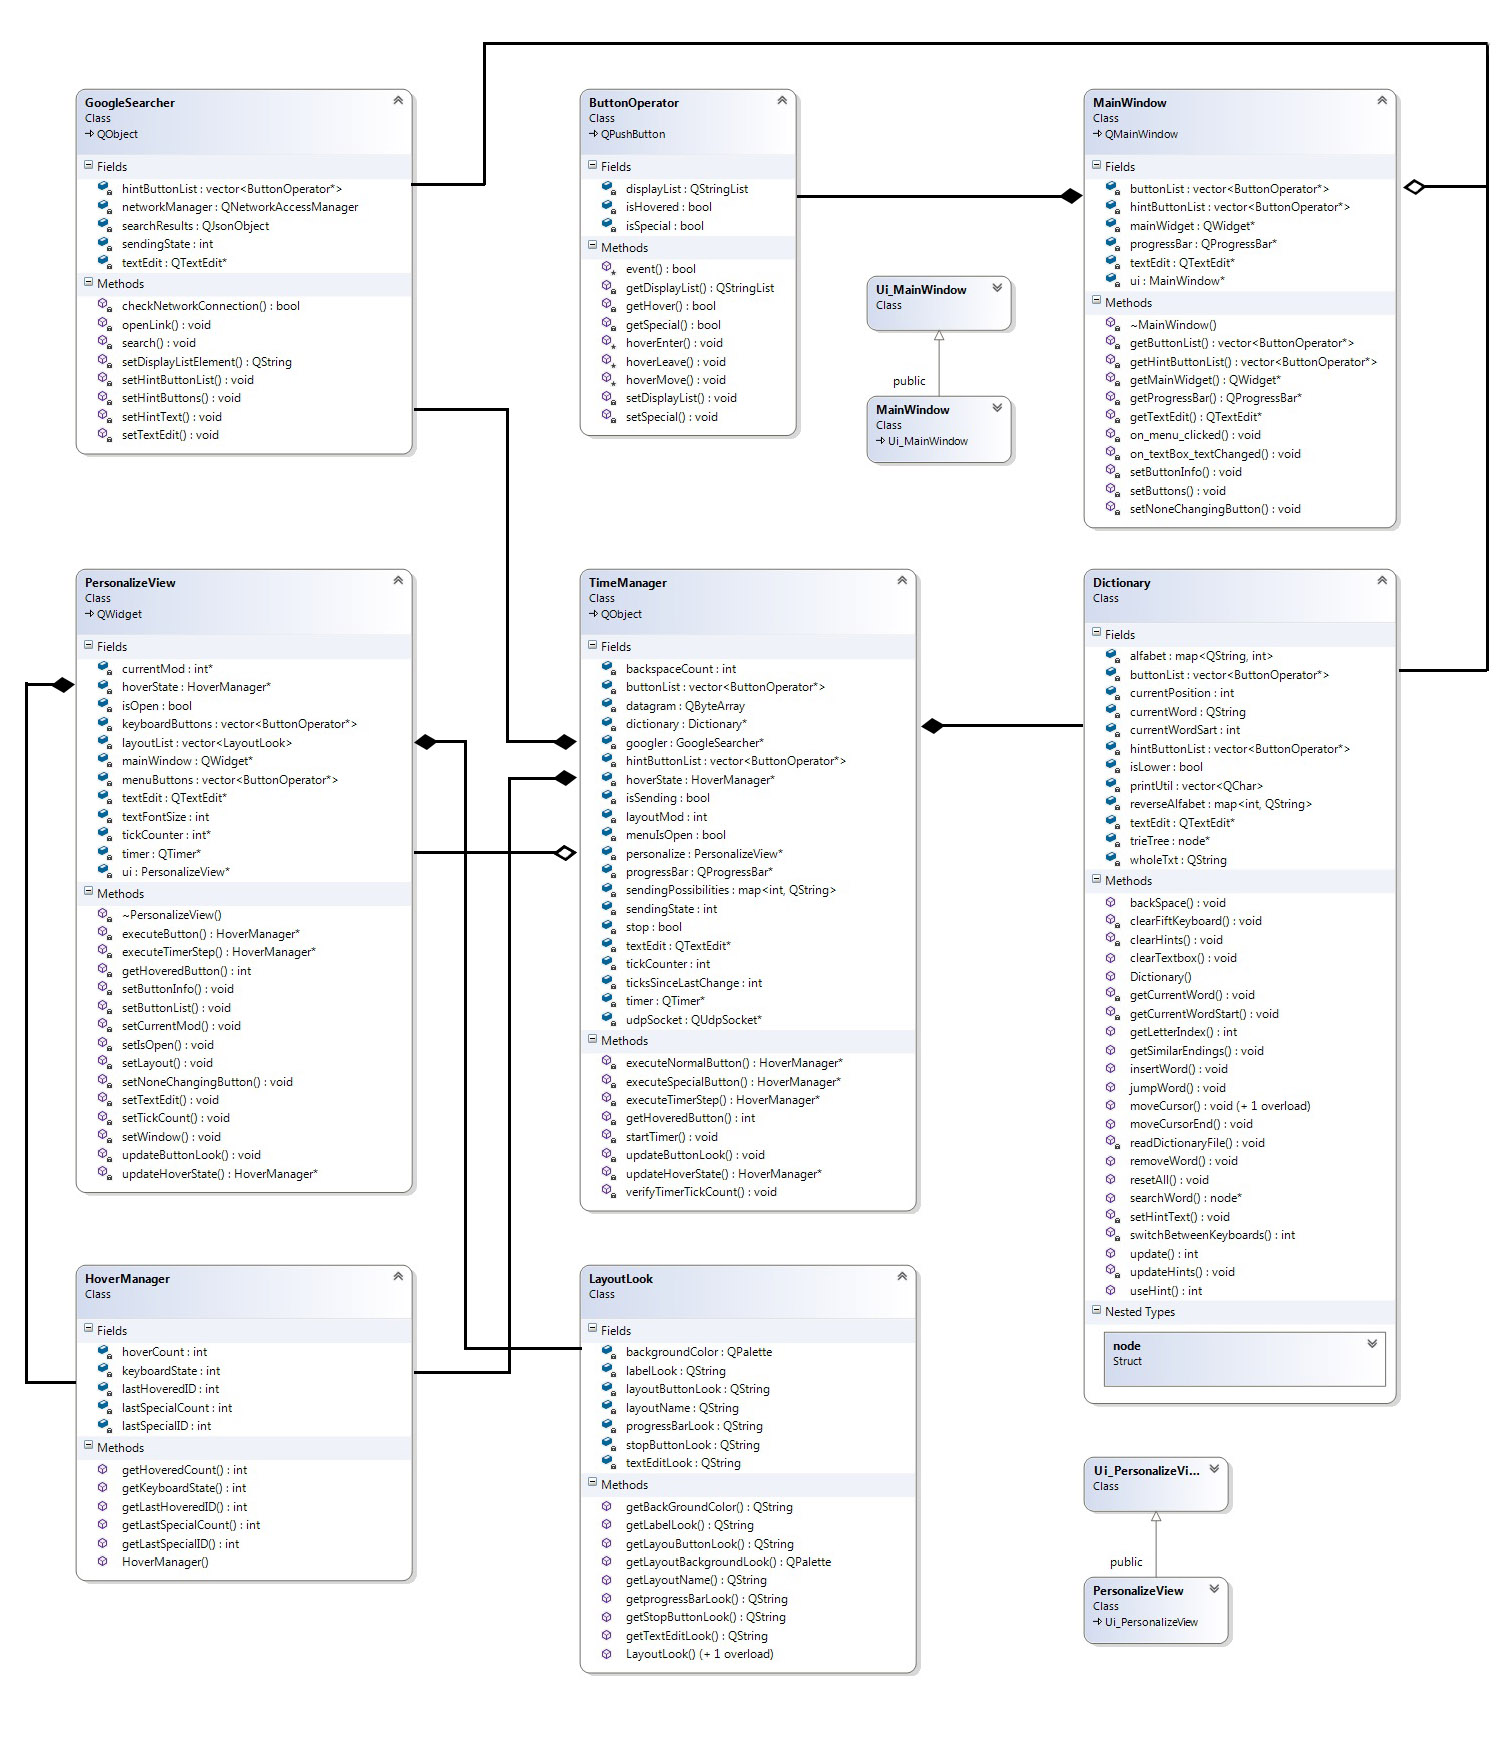
\includegraphics[width=0.7\textwidth]{img/classDiagram.jpg}}
		\caption{Poglądowy diagram klas zaimplementowanych w projekcie.}
		\label{fig:classDiag}
		
\end{figure}
\section{Opis klas zastosowanych}\label{sec:klas}
Klasami użytymi w programie są: ButtonOperator, Dictionary, GoogleSearcher, HoverManager, LayoutLook, MainWindow, PersonalizeView, TimeManager. Dla każdej z nich można określić główną funkcję. Zestawienie to przedstawiono w tabeli~\ref{table:classTab}.
\begin{table}
\renewcommand\arraystretch{1.5}
 \centering
    \begin{tabular}{|>{\centering\arraybackslash}m{4cm}|m{8.5cm}|}
     \hline
    \textbf{Nazwa klasy} & \textbf{Funkcja w programie}\\ \hline
     ButtonOperator& Klasa dziedzicząca po QPushButton (wewnętrzna klasa biblioteki QT) odpowiedzialna za działanie przycisków w projekcie.\\ \hline 
     Dictionary & Klasa zajmująca się pracą ze słownikiem, a także zarządzaniem wprowadzonym tekstem. Do kontruktora przyjmuje wskaźnik na pole tekstowe, listę wskaźników na wszystkie działające przyciski oraz listę wskaźników na przyciski odpowiedzialne za podpowiedzi. Klasa posiada również strukturę ''node'', która stanowi podstawowy element budulcowy dla słownika. Więcej na ten temat w podrozdziale ~\ref{sec:trietree}.  \\ \hline
     GoogleSearcher & Klasa zajmująca się komunikacją programu z internetem, obsługą rządania GET oraz przetworzeniem odpowiedzi. Więcej na ten temat w podrodziale ~\ref{sec:searcher}.\\ \hline
     HoverManager& Klasa nadzorująca działanie przycisków. Obiekty przechowują informację o: ID przycisku ostatnio fiksowanego, ID ostatnio wybranego specjalnego przycisku, czasie fiksacji nad jednym przyciskiem, czasem działania specjalnego przycisku. Więcej o przyciskach i ich działaniu w podrodziale ~\ref{sec:buttons}.\\ \hline
     LayoutLook& Klasa przewidziana z myślą o dynamicznej zmianie wyglądu przez użytkownika w oknie menu. Obiekty klasy zebrane w listę w klasie PersonalizeView przechowują komplet danych dotyczących jednego wyglądu. W skład tego wchodzą nazwa wyglądu, wygląd przycisków zapisany przy pomocy kaskadowego arkuszu styli, paletę zmieniającą kolor tła okien, arkusz styli dla paska postępu, podpisów oraz wyglądu przycisków w trybie zablokowanym.\\ \hline
     MainWindow& Gówna klasa projektu odpowiedzialna za komunikację interfejsu z resztą klas.\\ \hline
     PersonalizeView & Klasa odpowiedzialna za obsługę wszystkich zdarzeń związanych z okenm menu tzn. zmianą wyglądu aplikacji, zmianą wielkości czcionki, zmianą czasu progowego fiksacji.\\ \hline
     TimeManager & Rozbudowana klas będąca głównym zarządcą procesów zachodzących w aplikacji dzięki umiejętności pracy z regulatorem czasowym (timer). \\ \hline 
    
	\end{tabular}
	 \caption{Tabela przyporządkowania głownych funkji klasom projektu.} 
    \label{table:classTab}
\end{table}
\section{Zaimplementowane algorytmy}\label{sec:algorytmy}
W poniższych podrozdziałach zaprezentowano zasadę działania zaimple\-men\-towanych w oprogramowaniu algorytmów. 
\subsection{Działanie przycisków} \label{sec:buttons}
W aplikacji każdy przycisk jest obiektem klasy ButtonOperator, która dzie\-dzi\-czy po klasie QPushButton. Dzięki czemu obiekty przycisków mogą ko\-rzy\-stać zarówno z metod klasy nadrzędnej np. isCheckable(), jak i klasy dzie\-dzi\-czącej. Właśnie dzięki nadpisaniu metod domyślnych klasy QPushButton  -  ho\-ver\-Enter() i hoverLeave() stworzono możliwość detekcji, nad którym przyciskiem aktualnie znajduje się punkt fiksacji wzroku. Podczas wywołania obu metod zmieniana jest wartość logiczna zmiennej isHovered aktualnie obserwowanego przycisku.  Prócz informacji o tym, czy dany przycisk jest aktualnie używany przechowuje się również dane o tym, czy przycisk zalicza się do tzw. ''spe\-cja\-lnych'', czy też nie, jak i listę dostępnych dla niego tekstów do wy\-świe\-tla\-nia – wyglądów przycisku dla 6 stanów kla\-wia\-tu\-ry (małe litery, duże litery, znaki specjalne karta pierwsza, znaki specjalne karta druga, polskie litery, menu kontekstowe). Wszystkie te dane wprowadza się podczas  uruchamiania kla\-wia\-tu\-ry i wtedy także przypisuje się przyciski kolejno do specjalnej listy. Kolejność jest znacząca w przypadku przycisków ''specjalnych'', gdyż ich obsługa zależna jest od wartości ich ID zapisanego w pliku ze stałymi. 
Określenie przycisku działającego odbywa się poprzez sprawdzenie jego ID, którego zmienna isHovered jest prawdziwa w klasie TimeManager. Do zarządzania stanem kla\-wia\-tu\-ry, o\-sta\-tnio wybranym przyciskiem specjalnym oraz ostatnio obserwowanym przyciskiem powstała klasa HoverManager. Zbiera ona na bieżąco informację o  ID przycisku ostatnio najechanego, o tym przez jaki czas dany przycisk jest już pod punktem fiksacji, o aktualnym stanie kla\-wia\-tu\-ry, o os\-ta\-tnio wybranym spe\-cja\-lnym przycisku (np. CapsLock) oraz przez jaki czas działanie tego przycisku się utrzymuje. Większość z tych danych odświeżana jest co 200ms (stała zde\-fi\-nio\-wa\-na w pliku ze stałymi) podczas każdego wykonywania się metody TimerStep(). Jej działanie przedstawiono za pomocą pseudokodu ~\ref{sec:alg1}.
\begin{algorithm}
\caption{Działanie funkcji TimerStep()}
\label{sec:alg1}
\begin{algorithmic}
\STATE pobierz ID aktualnie fiksowanego przycisku
\IF{pobrane ID różne jest od -1}
\IF{zwykłe przyciski są w trybie wstrzymania}
\IF{jeśli aktualnie fiksowany przycisk jest specjalny}
\STATE hoverState (obiekt klasy HoverManager) ustaw aktualnie aktywny przycisk na pobrane ID
\STATE Wykonaj krok timera (funkcja executeTimerStep())
\STATE Pokaż czas przez jaki przycisk jest fiksowany na pasku postępu dla informacji użytkownika.
\ENDIF
\ELSE
\STATE Wykonaj powyższe funkcje dla wszystkich przycisków - niezależnie od tego, czy są specjalne, czy nie.
\ENDIF
\ENDIF
\STATE Wywołaj funkcję verifyTimerTickCount().
\end{algorithmic}
\end{algorithm}
\\Zadaniem wyżej wspomnianej funkcji \-executeTimerStep() jest sprawdzenie, czy dany przycisk był fiksowany przez odpowiednią ilość czas (zmienna, której wartość zależy od ilości pomyłek popełnionych przez użytkownika, jest dynamicznie zmieniana podczas korzystania z klawiatury – analizowane to jest w funkcji ve\-ri\-fyTimerTickCount()). Jeżeli warunek ten został spełniony to dalszy przebieg działań zależy od tego, czy przycisk był specjalny, czy też nie oraz czy klawiatura nie znajduje się w trybie wstrzymania. 
\subsubsection{Działanie przycisków specjalnych}
W tabeli ~\ref{table:specialButtons} wymieniono wszystkie specjalne przyciski z widoku klawiatury oraz opisano po krótce algorytm ich działania. W tabeli ~\ref{table:specialButtonsMenu} przedstawiono przyciski widoku menu oraz ich zachowanie.

\begin{table}
  \renewcommand\arraystretch{1.2}
 \centering
    \begin{tabular}{|>{\centering\arraybackslash}m{4cm}|m{8.5cm}|}
        \hline
    \textbf{Nazwa przycisku} & \textbf{Działanie}\\ \hline
     Backspace & Wywołuję metodą backspace() klasy Dictionary, której działanie opisano w podrozdziale ~\ref{sec:backspc}.\\ \hline
    CapsLock & W przypadku pierwszego wciśnięcia zmienia stan kla\-wia\-tu\-ry z 0 na 1 i utrzymuje ją dopóki nie zostanie wybrany po raz wtóry lub wykonana zostanie czynność innego przycisku zmieniającego stan klawiatury. \\ \hline
 Czyść & Korzysta z metody resetAll() klasy \-Dictionary i po\-wo\-du\-je czyszczenie edytora tekstowego oraz z nim związanych zmiennych jak currentPosition, currentWord, currentWordSart, wholeTxt (więcej na ten temat w rozdziale ~\ref{sec:text}).\\ \hline
Menu & Otwiera okno klasy Personalize.\\ \hline
Przesuń się o jedno słów w prawo lub w lewo & Wywołuje funkcje jumpWord() klasy Dictionary, która powoduje przesunięcie się kursora na koniec po\-prze\-dnie\-go słowa, lub na początek kolejnego. Każdorazowo zmieniana jest wartość zmie\-nnej currentWord i wholeText.~\ref{sec:text}\\ \hline
 Przesuń się w kierunku początku tekstu (home) lub na jego koniec (end) & Wybranie przycisku powoduje przesunięcie się kursora w jednym z dwóch kierunków oraz zmiane wartości zmie\-nnej wholeText i currentWord (~\ref{sec:text}). \\ \hline
 Przyciski podpowiedzi & Wyświetlane są na nich podpowiedzi, których tworzenie opisane jest w rodziale ~\ref{sec:trietree}. Ich użycie powoduje zastąpienie aktualnie wpisywanej frazy autouzupełnionym słowem pobranym ze słownika. \\ \hline
  Shift & W przypadku wciśnięcia zmieniony zostaje stan kla\-wia\-tu\-ry z 0 na 1, a po użyciu przycisku ze znakiem stan kla\-wia\-tu\-ry wraca do stanu 0. \\ \hline
   Stop i start & Wprowadza kla\-wia\-tu\-rę w stan wstrzymania lub w stan pracy. W zależności od wartości zmiennej isStop jest możliwe, lub nie, korzystanie z przycisków ze znakami.\\ \hline
   Strzałka w lewo i prawo &  Korzystając z metody moveCursor klasy Dictionary przemieszcza kursor o jeden znak w danym kierunku. Może zmienić wartość currentWord (~\ref{sec:text}) korzystając z metod getCurrentWord() oraz getCurrentWordStart()(~\ref{sec:alg2}) opisanych w późniejszych rozdziałach.\\ \hline
     Wyjdź & Powoduje opuszczenie aplikacji.\\ \hline 
      Wyszukaj na podanej platformie & Przyciśniecie przycisku powoduje sprawdzenie połączenia internetowego, a następnie wysłanie wpisanej treści pola tekstowego do funkcji search() klasy GoogleSearcher. ~\ref{sec:searcher}\\ \hline
        Wyślij & Wysyła dotychczas wpisany tekst na broadcast na port 45454 za pomocą metody writeDatagram() klasy QUdpSocket.\\ \hline
    Zmiana trybu wyszukiwania & Strzałki powodują na zmianę trybu wyszukiwania. Do wyboru ''Google'', ''YouTube'', ''Filmweb''. Zmieniają wartość zmiennej sendingState niezbędnej do popranego działania funkcji  search() klasy GoogleSearcher.~\ref{sec:searcher}\\ \hline 
    Znaki specjalne & Zmienia stan kla\-wia\-tury na odpowiednio 2 i 3 przy ko\-lej\-nych kliknięciach. \\ \hline
       \end{tabular}
    \caption{Lista specjalnych przycisków wraz z ich działaniem.} 
    \label{table:specialButtons}
\end{table}
\begin{table}
   \renewcommand\arraystretch{1.5}
 \centering
    \begin{tabular}{|>{\centering\arraybackslash}m{4cm}|m{8.5cm}|}
        \hline
    \textbf{Nazwa przycisku} & \textbf{Działanie}\\ \hline
       Strzałki zmieniające aktualną wartość progową czasu fiksacji & Strzałki powodują zmniejszenie lub zwiększenie wartości zmiennej tickCounter przechowującej ilość 200ms interwałów, po upływie których (w przypadku braku zmiany fiksowanego punktu) przycisk można uznać za wciśnięty. Początkowo czas ten wynosi 3s, jednak w wyniku dynamicznej korekty następuje zmniejszenie lub zwiększenie liczby tych interwałów. Korekta uruchamia się, gdy użytkownik przekroczy dopuszczalną ilość błędów w ciągu minuty. Więcej na temat dynamicznej zmiany czasu w podrozdziale ~\ref{sec:dynamic}. \\ \hline  
       Strzałki zmieniające wielkość czcionki w edytorze tekstu & Strzałki powodują zamianę właściwości edytora tekstu. \\ \hline
       Strzałki zmieniające wygląd aplikacji & Użytkownik może wybrać między jednym z 5 wersji kolorystycznych poprzez dynamiczną zmianę wyglądu na podstawie danych z listy i aktualnego indeksu.  \\ \hline    
       Wyjście & Powoduje zamknięcie okna menu. \\ \hline
    \end{tabular}
    \caption{Lista specjalnych przycisków z menu w raz z ich działaniem.} 
    \label{table:specialButtonsMenu}
\end{table}
Jako wciśnięcie rozumie się tu czas fiksacji nad przyciskiem przekracający progową wartość. Stany klawiatury to odpowiednio 0-małe litery, 1-wielkie litery, 2-znaki specjalne strona pierwsza, 3-zanki specjalne strona druga,\\4-polskie znaki, 5-menu kontekstowe dla polskich znaków.
\subsubsection{Działanie przycisków nomalnych}
Za wpisywanie znaków z klawiatury do edytora odpowiedzialna jest funkcja \-update() klasy Dictionary. Jest ona głównym zarządcą jeśli chodzi o wprowadzanie znaków w odpowiedniej pozycji. W pierwszej kolejności sprawdzane jest, czy stan klawiatury różny jest od stanu piątego (menu kontekstowe). Gdy spełniony jest dany warunek to porównywana jest aktualnie wprowadzana wartość z u\-prze\-dnio wprowadzoną. Wyjątek stanowi pierwsze wprowadzenie znaku do e\-dy\-to\-ra. W przypadku dwóch identycznych liter czyszczona jest zawartość piątego stanu klawiatury i przechodzi się do wywołania funkcji switchBetweenKeyboards(), która zwraca informację o tym, czy stan kla\-wia\-tu\-ry się zmienił. Tam sprawdzane jest, czy wprowadzony znak jest jedną z liter posiadających polskie odpo\-wie\-dni\-ki tj. \textit{a-ą, c-ć, e-ę, l-ł, n-ń, o-ó, s-ś, z-ż-ź}. Gdy znajdzie się on wśród wymienionej listy, to dla odpowiadającego przycisku ustawiany jest test dla klawiatury stanu piątego i następuje jej wyświetlenie. Działanie takiego zachowania widać na rysunkach 
 ~\ref{fig:startA},~\ref{fig:doubleA}.
\begin{figure}
		\centering
		\scalebox{.7}{
		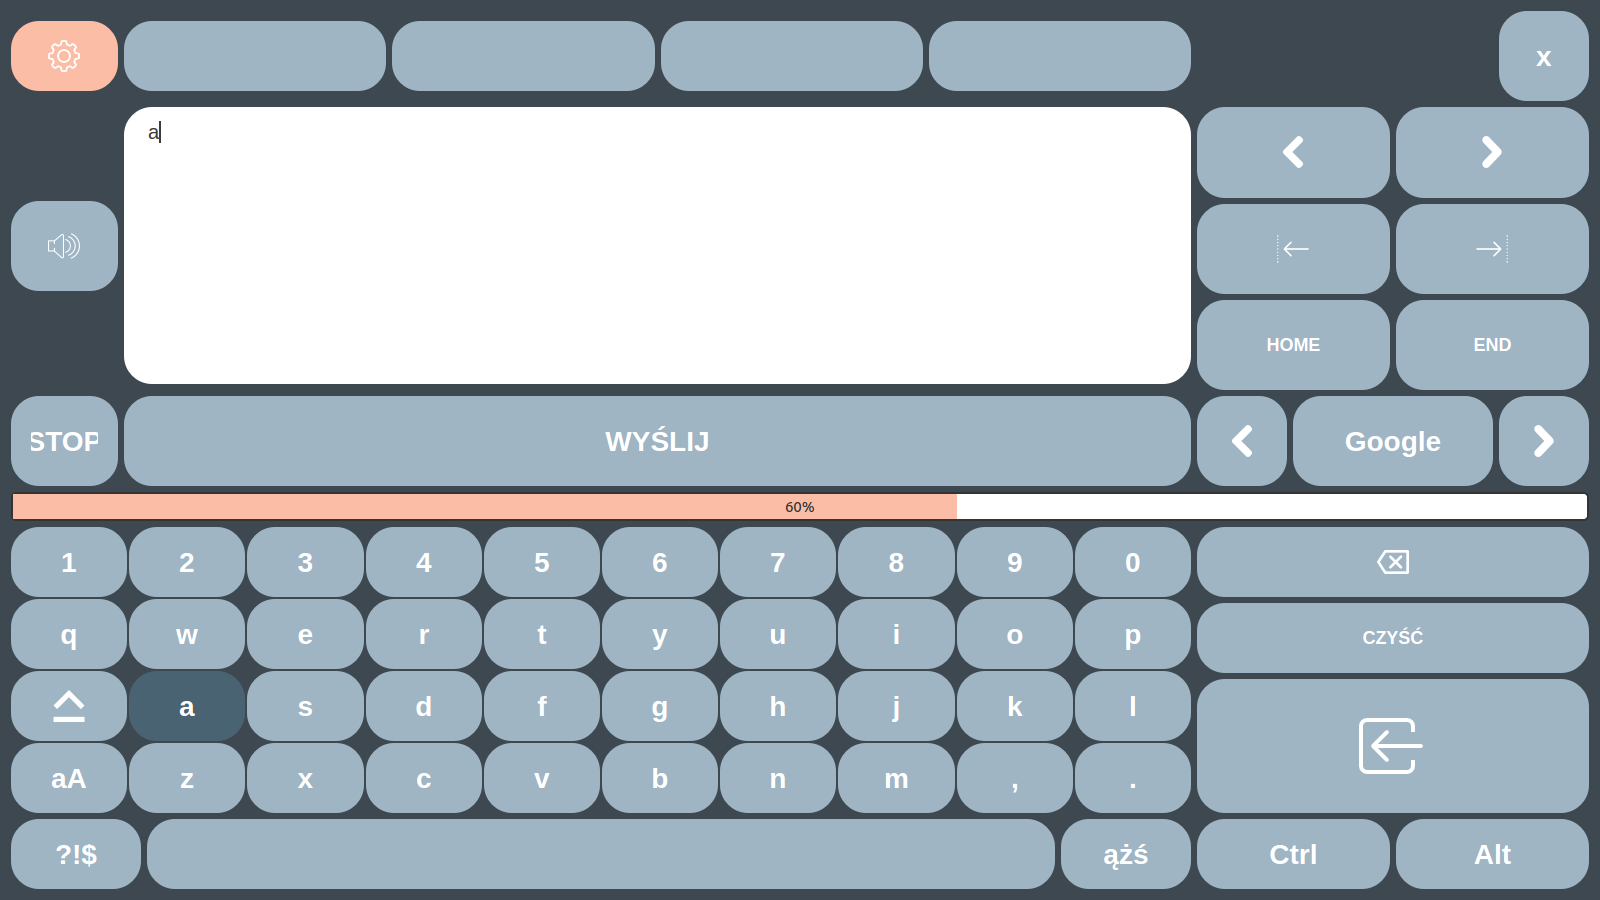
\includegraphics[width=1\textwidth]{img/startA.jpg}}
		\caption{Widok aplikacji z klawiatura w stanie zerowym po wpisaniu litery 'a'.}
		\label{fig:startA}
\end{figure}
\begin{figure}
		\centering
		\scalebox{.7}{
		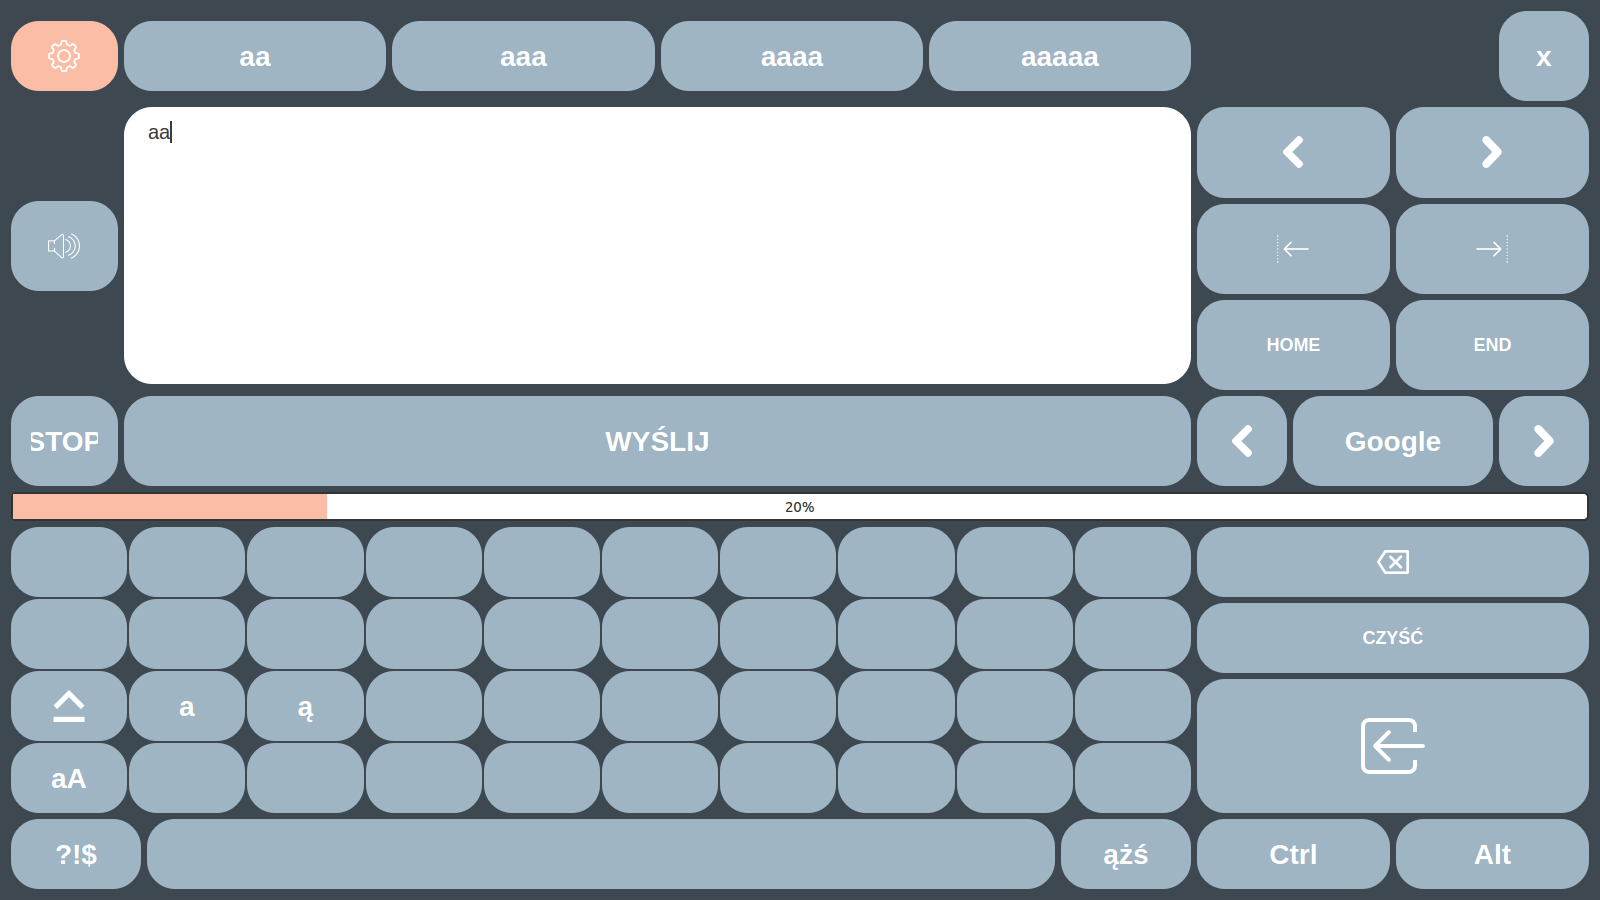
\includegraphics[width=1\textwidth]{img/doubleA.jpg}}
		\caption{Widok aplikacji z klawiaturą w stanie piątym po wpisaniu drugiej litery 'a'.}
		\label{fig:doubleA}
\end{figure}\\
W innym wypadku aktualna litera dopisywana jest do aktualnie tworzonoego słowa (currentWord), kursor przesuwany jest o jedną pozycję w prawo. Gdy dodana jest spacja aktualnie przetwarzane słowo jest uznawane za skończone i zapamiętywany jest nowy początek kolejnego słowa. Odświeżony zostaje również widok podpowiedzi, których powstawanie omówiono w późniejszym rozdziale ~\ref{sec:trietree}.
W sytuacji, gdy wybrana zostaje litera z menu kontekstowego (klawiatury w stanie piątym), to albo wpisany tekst zostaje podmieniony na polską literę,lub nie ulega zmianie. Przykładowo po wpisaniu ''aa'' użytkownik po raz kolejny wybiera literę ''a'' - tzn. planował wpisanie frazy ''aa''. Jeśli jednak decyduje się na literę ''ą'', to w miejsce widniejącego napisu ''aa'' pojawia się ''ą''.
Poglądowy diagram przepływu przedstawiono no rysunku ~\ref{fig:wordFlow}.
\begin{figure}[!h]
		\centering
		\scalebox{1}{
		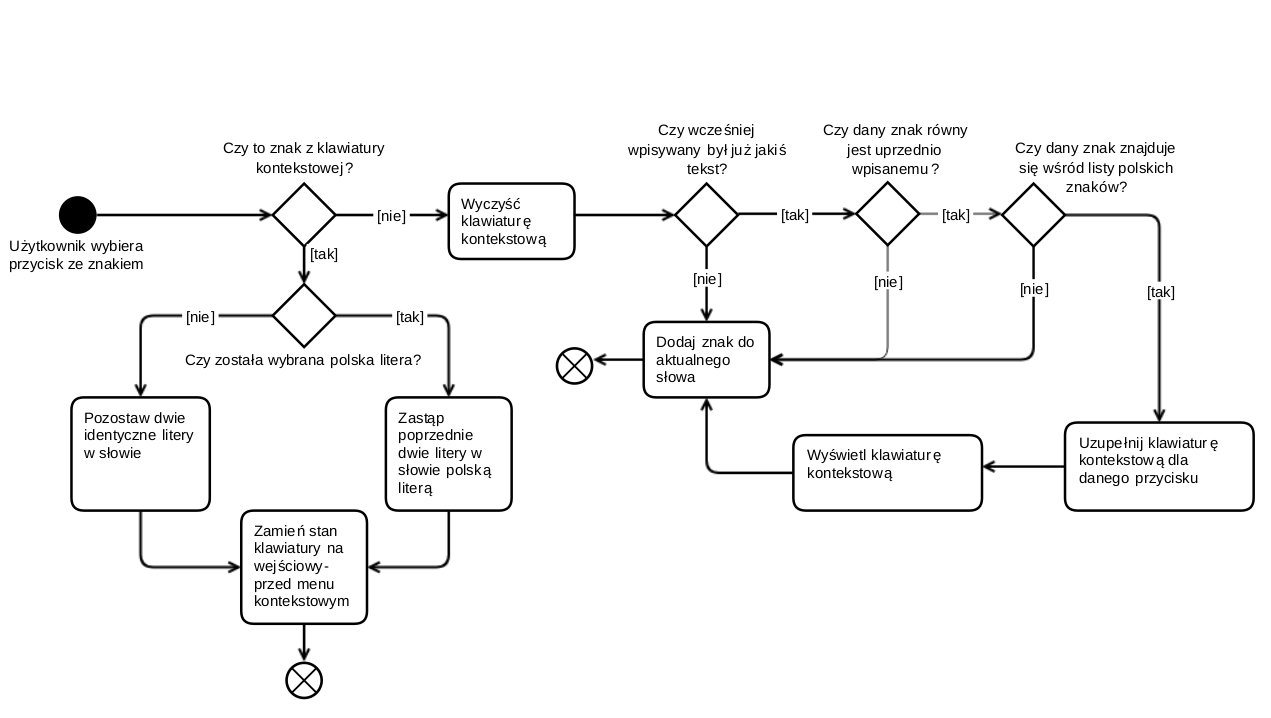
\includegraphics[width=1\textwidth]{img/writeFlow.jpg}}
		\caption{Widok aplikacji z klawiaturą w stanie piątym po wpisaniu drugiej litery 'a'.}
		\label{fig:wordFlow}
\end{figure}
\subsection{Praca z tekstem}~\label{sec:text}
Wpisywanie tekstu w aplikacji odbywa się poprzez specjalny algorytm kontrolujący zawartość aktualnie pisanego słowa oraz całego tekstu. W czasie działania programu, w pamięci przechowywany jest currentWord, czyli aktualne słowo tj. ciąg znaków, liter lub cyfr, które zaczynają się na początku wpisywanego tekstu lub po spacji, a kończą się w pozycji kursora. Dodanie spacji po ciągu znaków kończy słowo i usuwa je ze zmiennej currentWord, a dodaje do zmiennej zwanej wholeText, która przechowuje dotychczas wpisany tekst. Przykładowo jeśli mamy tekst jak na rysunku ~\ref{fig:sentence} to w zmiennej wholeText przechowywujemy ''''Wymagajcie od siebie choćby inni od was nie wymagali.'' ~Jan Paweł II '', a w currentWord ''sie''. W ten sposób podpowiedzi generowane będą jedynie dla cząstki ''sie'', a tekst wpisywany będzie w pozycji kursora, która również monitorowana jest przez zmienną currentPosition. Scalenie wholeText i currenWord następuję, gdy zmieniamy pozycję kursora strzałkami, lub jeśli do tekstu dodana zostanie spacja, a za kursorem nie znajduje się żaden znak. Przykład przedstawia rysunek ~\ref{fig:sentence2}. 
\begin{figure}[!h]
		\centering
		\scalebox{1}{
		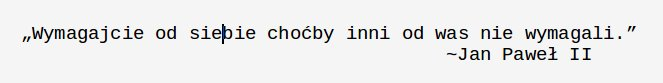
\includegraphics[width=1\textwidth]{img/sentence.jpg}}
		\caption{Przykładowe zapisywanie tekstu do zmiennych w zależności od pozycji kursora.}
		\label{fig:sentence}
\end{figure}
\begin{figure}[!h]
		\centering
		\scalebox{1}{
		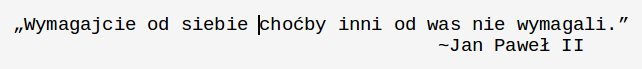
\includegraphics[width=1\textwidth]{img/sentence2.jpg}}
		\caption{Przykładowe zapisywanie tekstu do zmiennych w zależności od pozycji kursora.}
		\label{fig:sentence2}
\end{figure}

Zmienna currentWord została zespolona z wholeText poprzez wklenie jej na pozycji zapisanej jako currentWordStart. 
W celu dynamicznego ustalania pozycji currentWordStart oraz zawartości currentWord powstały funkcje: getCurrentWordStart() oraz getCurrentWord(). Działanie pierwszej zademonstrowano za pomocą pseudokodu ~\ref{sec:alg2}.
\begin{algorithm}
\caption{Działanie funkcji getCurrentWordStart()}
\label{sec:alg2}
\begin{algorithmic}
\IF{currentWord nie jest pusty \&\&  currentPosition nie jest  na początku tekstu}
\FOR{każda pozycja aż do początku tekstu}
\STATE pobierz literę z wholeText w danej pozycji
\IF{pobrana wartość nie jest liczbą ani literą}
\STATE $currentWordStart = dana pozycja + 1$
\ENDIF
\ENDFOR
\ENDIF
\end{algorithmic}
\end{algorithm}\\
Działanie drugiej sprowadza się do wycięcia faragmentu tekstu między currentWordStart, zaimplementowanym w wyniku działania poprzedniej funkcji, a currentPosition.
\subsubsection{Usuwanie znaków} \label{sec:backspc}
Proces usuwania znaków staje się trudniejszy ze względu na ułatwiające kontrolę nad tekstem currentWord i wholeText. Pier\-wszym napotkanym problemem była sytuacja, w której currentWord jest puste. W takim wypadku należy usunąć znak znajdujący się w currentPosition ze zmie\-nnej wholeText, a następnie za pomocą wcześniej opisanych funkcji getCurrentWordStart() oraz getCurrentWord() otrzymać informację o nowej wartości currentWord. Kolejnym krokiem jest wycięcie wartości zmiennej currentWord z wholeText, przesunięcie kursora dla informacji użytkownika w odpowiednią pozycję oraz odświeżenie wyglądu podpowiedzi.
Gdy currentWord ma wartość, sytuacja upraszcza się do usunięcia ostatniego znaku z currentWord. W celu reprezentacji tekstu dla użytkownika należy scalić wholeText z currentWord, ale by nie utracić wartości wholeText stworzono tymczasową zmienną currentText, który zawiera całą treść wpisanego tekstu.
\subsection{Trie tree}\label{sec:trietree}
Jak wyżej ~\ref{sec:trie}  wspomniano, w pracy wykorzystano drzewo typu Trie w celu pracy z rozległym słownikiem. Słowa z pliku w formacie TXT wczytywane są do programu podczas uruchamiania klawiatury- każda z linii dostarczanego pliku powinna stanowić pojedynczy wyraz. Słowa te, za pomocą sztucznie wy\-ge\-ne\-ro\-wa\-nych list kodujących oraz dekodujących polski alfabet, wprowadzane są do drzewa typu Trie. Drzewo takie powstaje poprzez stworzenie pustego węzła typu node - struktury zadeklarowanej w pliku nagłówkowym klasy obsługującej współpracę ze słownikiem – Dictionary. Struktura node przechowuje informacje o rodzicu bieżącego węzła, o jego potomkach – czyli węzłach następujących oraz wektor zawierający informację o przynależności danego węzła literowego do słowa. 
Po zainicjowaniu węzła zerowego, po kolei analizowane są słowa ze sło\-wni\-ka w funkcji insertWord().Każde jest rozpatrywane jako tablica liter (char) \\i iteracyjnie następuje najpierw kodowanie litery na odpowiadający jej indeks (za pomocą  mapy alfabet), potem, sprawdzane jest, czy w drzewie nie istnieje już węzeł odpowiadający danej wartości. Gdy nie znaleziono gałęzi drzewa pasujących do poszukiwanej wartości tworzy się za pomocą funkcji calloc przestrzeń w pamięci na przyszłe dzieci tego węzła, a jako ich rodzica podaje się aktualnie przeglądany węzeł z literą. Kolejno, niezależnie od wyniku uprzednio rozpatrywanego warunku, o ile słowo wciąż posiada litery do przeglądu, przenosi się \\o poziom niżej w drzewie ( na poziom dziecka  uprzednio rozpatrywanej litery) \\i proces zachodzi od początku.  Gdy przetworzono wszystkie litery słowa do listy wystąpień ostatniego odwiedzonego węzła dopisany zostaje indeks słowa \\w słowniku – tym samym oznaczając jego koniec. Na rysunku ~\ref{fig:insertWord} przed\-sta\-wio\-no, w sposób graficzny, działanie danej funkcji.
\begin{figure}[!h]
		\centering
		\scalebox{1}{
		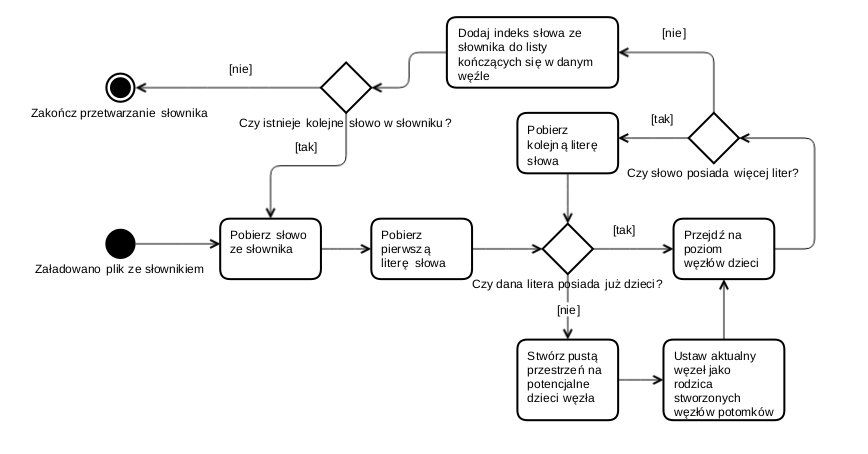
\includegraphics[width=1\textwidth]{img/insertWordFlow.jpg}}
		\caption{Diagram przepływu dla funkcji insertWord() wprowadzającej słowa do drzewa typu Trie. }
		\label{fig:insertWord}
\end{figure}

Po uzupełnieniu słownika nastąpić może autouzupełnianie wpisywanego tekstu.
Każde wpisanie litery powoduje wywołanie metody updateHints(), która jest odpowiedzialna za tworzenie oraz wyświetlanie podpowiedzi, zgodnie \\z wprowadzonym do tej pory słowem. Jako poszukiwaną frazę traktujemy ciąg znaków, które użytkownik wpisał do pozycji kursora od ostatniej spacji, bądź początku tekstu. W wypadku, gdy ten ciąg znaków jest dłuższy niż dwa, wykorzystywana jest funkcja komunikująca się ze stworzonym słownikiem – searchWord(). Przekazywane jest drzewo Trie słownika oraz aktualnie poszukiwana fraza (bez formatowania). 
Wpisywana fraza, również traktowana jest jako zbiór liter, które przeglądane są jedna po drugiej. Dla każdej następuje zmiana dzięki mapie kodującej alfabet na odpowiadający indeks, który umożliwia przeszukiwanie słownika. Sprawdzane jest, czy istnieje potomek drzewa Trie o danym indeksie – jeśli tak, to następuje zmiana węzła na węzeł dziecka, tak, że przy przeszukiwaniu drzewa będą brane pod uwagę jedynie węzły z rodzicem będącym pierwszą literą poszukiwanej frazy. Gdy przeszuka się wszystkie litery, bądź w trakcie tego procesu zabraknie węzłów potomków dla danej kombinacji liter to zwracany jest odpowiednio ostatni węzeł wspólny dla danej frazy lub też węzeł pusty. 

W celu lepszego zrozumienia działania algorytmu rozpatrzmy go na przykładzie. Załóżmy, że mamy drzewo takie jak na rysunku ~\ref{fig:trie}. Jeśli wyszukamy frazę ''ko'' to funkcja zwróci nam węzeł i jego dzieci. Możliwe autouzupełnienia wyglądają wtedy tak jak na rysunku ~\ref{fig:trieKO}.
\begin{figure}[!h]
		\centering
		\scalebox{.5}{
		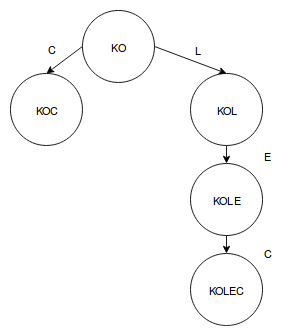
\includegraphics[width=1\textwidth]{img/trieKO.jpg}}
		\caption{Przykładowy węzeł do autouzupełniania słów po wpisaniu frazy ''ko''. }
		\label{fig:trieKO}
		\end{figure}
Złożenie końcówek wyrazów zachodzi w funkcji getSimilarEndings(), której przekazywany jest znaleziony
 węzeł, pusty wektor, do którego mają zostać zapisane wynikowe wyrazy oraz węzeł znaków niezbędny do dekodowania. 
W pierwszym kroku sprawdzane jest, czy w danym węźle kończą się  jakieś słowa, jeśli tak (wektor wystąpień węzła jest różny od zera), \\to każdą literę zapisaną w wyżej wymienionym wektorze znaków zapisuje się do jednego słowa (tworząc końcówkę do autouzupełniania). Gotowy ciąg znaków zapisywany jest do wektora z końcówkami. W wypadku pierwszego wykonania się funkcji mamy do czynienia z pustym wektorem znaków- toteż nie zostanie stwo\-rzo\-na żadna końcówka. Nawet jeśli  ‘’ko’’ było pełną formą słowa nie powinna się ona wyświetlać w proponowanych opcjach użytkownika. Aby uzupełnić we\-ktor znaków należy przejrzeć przesłany węzeł (ten z rysunku ~\ref{fig:trieKO}) – w tym celu sprawdza się, czy dzieci węzła odpowiadającej każdej literze alfabetu nie są puste, gdyż programowe drzewo ma, prócz wcześniej przedstawionych gałęzi, jeszcze 33 (zakładając, że zaimplementowany alfabet posiada 35 liter) nieobdarzone wartością gałęzie przedstawione na rysunku ~\ref{fig:trieKOnull}. Gdy znaleziono element o niezerowej wartości pobierana jest za pomocą mapy symetrycznej (reverseAlfabet) wartość literowa węzła i wprowadzana jest do wektora znaków. Węzeł z ‘’ko’’ zmieniany jest w węzeł pierwszego pierwszego dziecka – w tym wypadku ‘’koc’’. Następnie przez rekurencję ponownie rozpoczyna się sprawdzanie, czy dane słowo kończy się w tym węźle. Jeśli tak, to proces zachodzi według powyżej opisanych kroków, jeśli nie, to znów poszukiwany jest węzeł potomny z kolejną literą końcówki słowa do autouzupełniania. Algorytm przedstawiono w sposób graficzny na rysunku ~\ref{fig:similarEndingsFlow}
		\begin{figure}[!h]
		\centering
		\scalebox{.9}{
		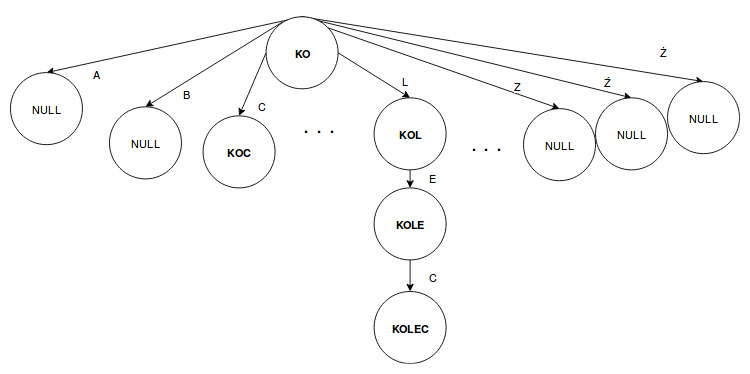
\includegraphics[width=1\textwidth]{img/trieKOnull.jpg}}
		\caption{Reprezentacja przykładowego węzła widzianego w programie. }
		\label{fig:trieKOnull}
		\end{figure}
				\begin{figure}[!h]
		\centering
		\scalebox{1}{
		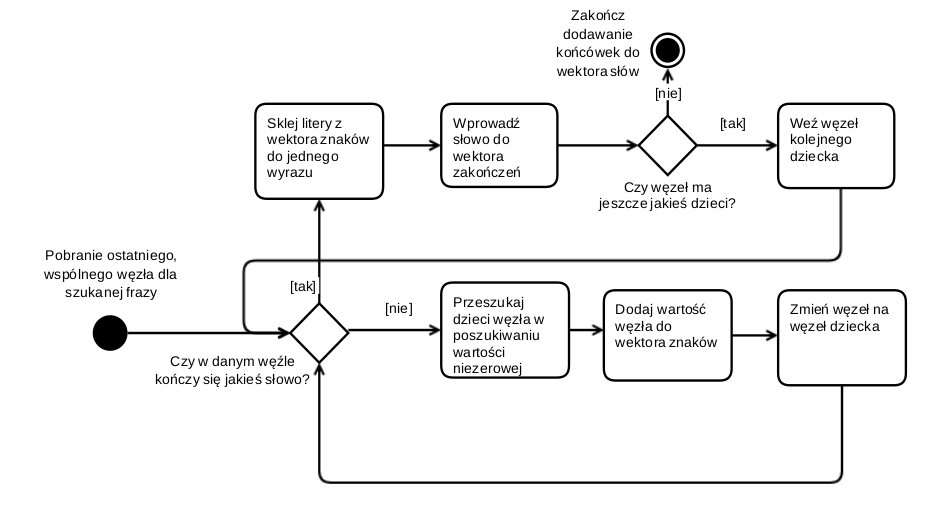
\includegraphics[width=1\textwidth]{img/similarEndingsFlow.jpg}}
		\caption{Diagram przepływu dla funkcji getSmiliarEndings().}
		\label{fig:similarEndingsFlow}
		\end{figure}\\
Ostatnim krokiem w stworzeniu podpowiedzi jest skrócenie listy końcówek do liczby przycisków przeznaczonych na podpowiedzi oraz zespolenie ich z dotychczas wpisanym słowem. Taki ciąg znaków można przedstawić użytkownikowi jako napis na przycisku, który po wybraniu wpisuje reprezentowany tekst do pola tekstowego zamieniając dotychczasową frazę na wybraną oraz dodając znak spacji na końcu nowowybranego słowa.
\subsection{Dynamiczna zmiana czasu progowego fiksacji}\label{sec:dynamic}
Jak wspomniano wcześniej klawiatura umożliwia dynamiczną zmianę czasu czasu progowego fiksacji (decydującego o tym kiedy dany przycisk zostanie wywołany). Zmiana następuję w oparciu o ilość błędów wykonanych przez użytkownika w określonym oknie czasowym. Weryfikacja następuję co minutę. Jeśli w tym czasie użytkownik popełni 5 lub więcej błedów (użyje przycisku Backspace), to czas fiksacji ulegnie wydłużeniu o jedną sekundę. Pięć błedów stanowi, dla ustawień początkowych, czyli progowego czasu fiksacji ustawionego na 3s, 25\% znaków wpisanych w tym czasie. Dla ilości błędów mniejszej niż dwa czas fiksacji zostaje skrócony. Jeśli użtkownik użyje przycisku Backspace 3-4 razy w ciągu minut czas progowy fiksacji nie ulegnie zmianie. Czas fiksacji został ograniczony obu\-stro\-nnie poprzez stałe z pliku const.h. Założono, że nie może on być krótszy niż 1s i dłuższy niż 6s. Użytkownik ma również możliwość manualnego ustawienia czasu progowego, poprzez zmianę wartości w oknie menu.  

\subsection{Korzystanie z wyszukiwarki internetowej}\label{sec:searcher}
W celu pracy z przeglądarką niezbędne jest podłączenie drugiego ekranu, na którym może się otwierać okno przeglądarki. W innym wypadku okno kla\-wia\-tu\-ry ulegnie minimalizacji i nie ma możliwości powrotu do okna.

W przypadku skorzystania z jednego z trybów wysłania (''Google'', \\''YouTube'', ''Filmweb'') wywoływana jest metoda, GoogleSearcher, search(). W zależności od przesłanej wartości sendingState, informującego o tym, gdzie wysłane ma być zapytanie, do wyszukiwanego tekstu (pobranego z pola tekstowego) dołączana jest informacja, w którym serwisie szukać wyników. Taka informacja załączana jest jako argument uzupełniający URL powstały przez stworzenie spersonalizownej wyszukiwarki, dzięki spe\-cja\-lne\-mu Google API. Następnie obiekt klasy QNetworkAccessManager wywołuję metodę RESTową GET na obiekcie klasy QNetworkRequest, który za argument konstruktora przyjmuje powstałe URL z paramatrem.
\subsubsection{Google Api}
Jak już wcześniej wspomniano ~\ref{sec:customSearch} do projektu wykorzystano specjalne API Google - Google Custom Search Engine. Dzięki temu powstał specjalny link URL umożliwiający przyjmowanie różnych parametrów jako zapytanie do wyszukiwaraki. Co więcej specjalne API na rządanie GET zwraca iformację w postaci QNetworkReply, gdzie funkcja handleNetworkData() umożliwia jego przetworzenie w ustrukturyzowaną postać JSON. Obiekt JSON zawiera 10 pierwszych wynków wyszukiwania w specjalnej przeglądarce. Każdy z obiektów typu JSON posiada informacje o wyniku wyszukiwania. W skład takiego obiektu wchodzą ~\cite{googleJSON}:
\begin{itemize}
\item ''kind'': ''customsearch\#result''
\item ''title'': string
\item ''htmlTitle'': string
\item ''link'': string
\item ''displayLink'': string
\item ''snippet'': string
\item ''htmlSnippet'': string
\item  ''cacheId'': string
\item ''mime'': string,
\item ''fileFormat'': string
\item ''formattedUrl'': string
\item ''htmlFormattedUrl'': string
\item ''pagemap''
\end{itemize} 
Wykorzystując dane z ''title'' oraz ''link'' przedstawiane są użytkownikowi cztery pierwsze wyniki wyszukiwania w polu tekstowym,a ich wywołanie (otworzenie strony) odbywa się przez wybranie przystosowanych przycisków podpowiedzi \\z numerem wyniku wyszukiwania w przypadku wyszukiwania danych w Google. Przykład działania przedstawiono na rysunkach ~\ref{fig:googleSearch} oraz ~\ref{fig:searchResult}. 
			\begin{figure}[!h]
		\centering
		\scalebox{.7}{
		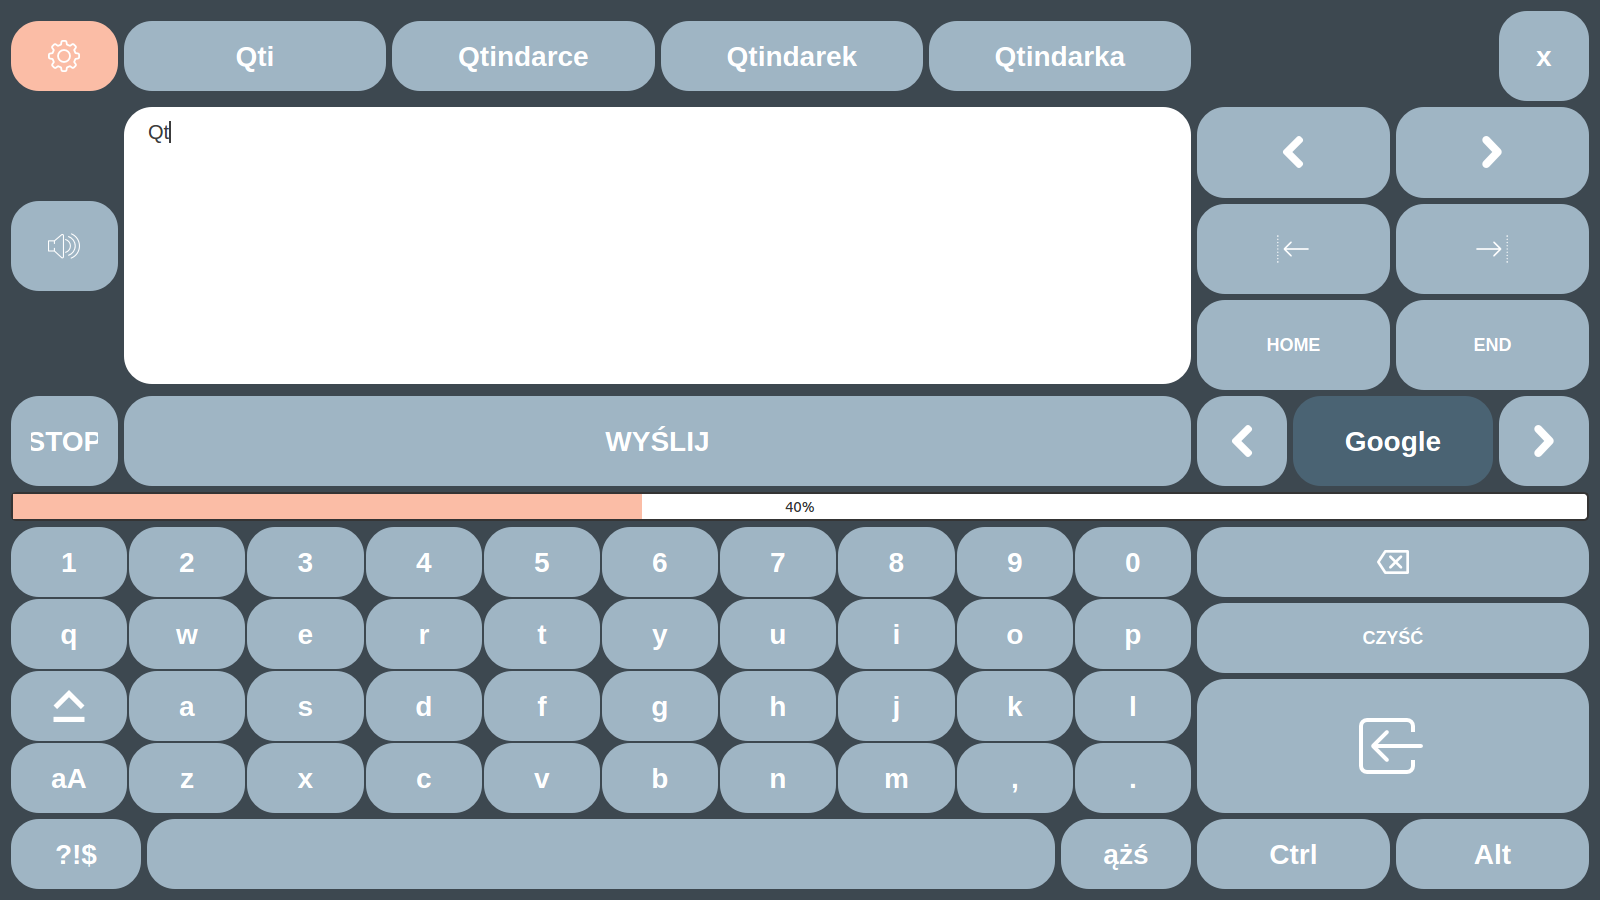
\includegraphics[width=1\textwidth]{img/qtSearch.jpg}}
		\caption{Przykładowy tekst wpisany do pola tekstowego, wysyłany jako argumnet wyszukiwania Google.}
		\label{fig:googleSearch}
		\end{figure}

	\begin{figure}
		\centering
		\scalebox{.7}{
		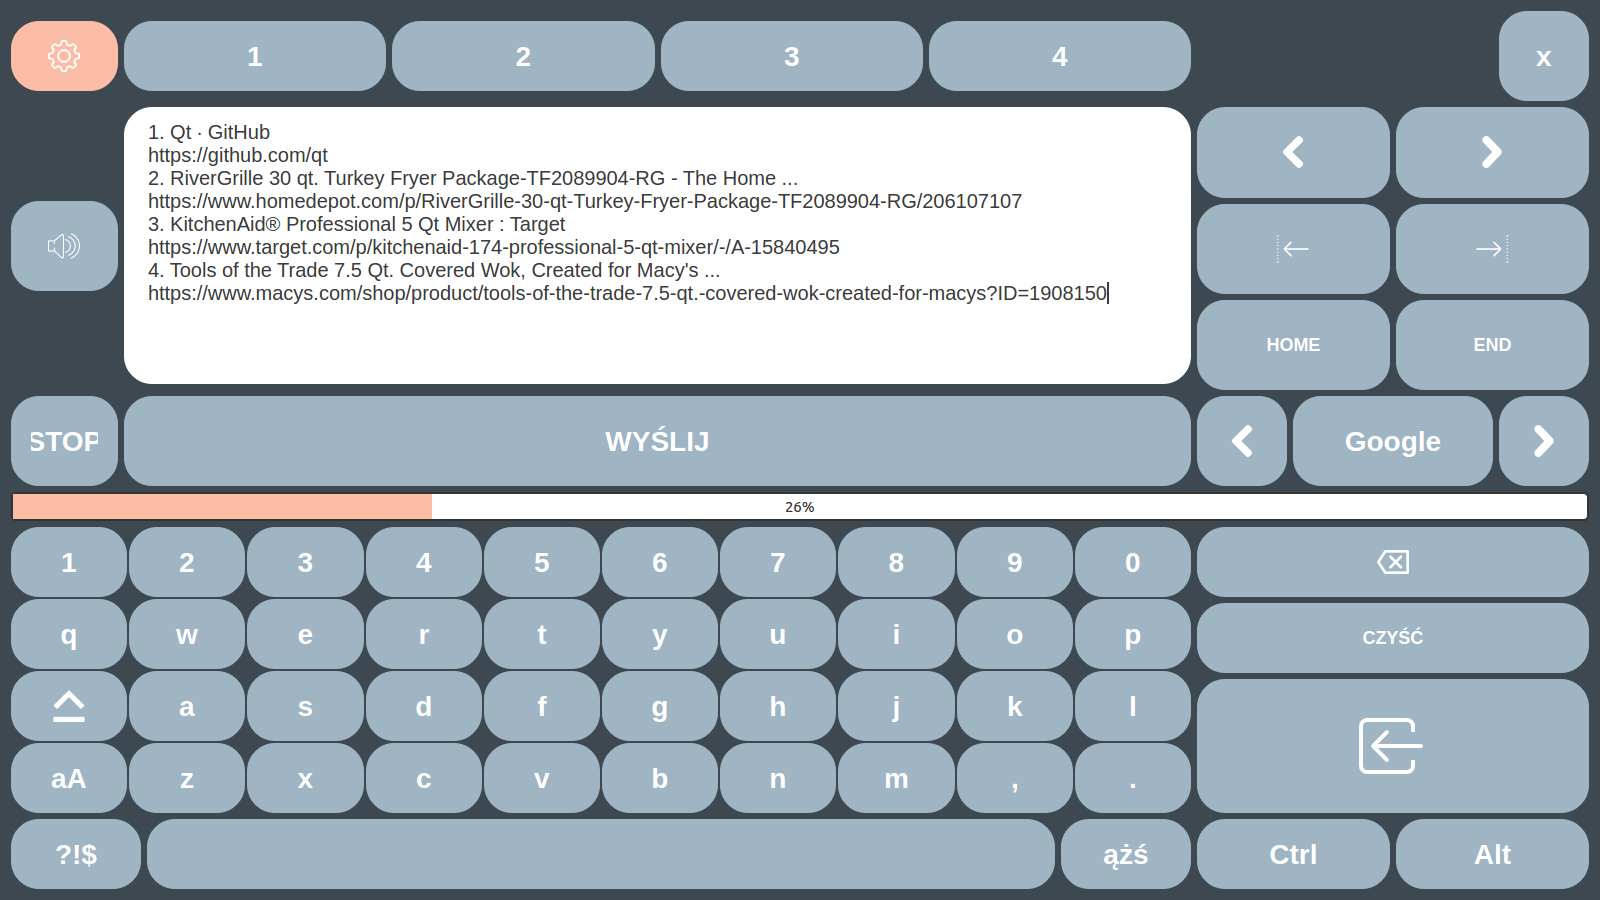
\includegraphics[width=1\textwidth]{img/qtsearchResult.jpg}}
		\caption{Wyniki wyszukiwana tekstu wpisanego na rysunku ~\ref{fig:googleSearch}.}
		\label{fig:searchResult}
		\end{figure}
W wypadku wyszukiwań w Youtube oraz Filmweb użytkownik nie ma możliwości wyboru  wyniku wyszukiwania - otwierany jest pierwszy wynik, który zawiera odpowiednie słowa kluczowe.
\section{Zaimplementowany interfejs użytkownika}
Zaimplementowany interfejs użytkownika uległ przemodelowaniu w porównaniu z przedstawionym wcześniej projektem.~\ref{sec:key} Wygląd nowego interfejsu można zaobserwować na rysunkach ~\ref{fig:view1}, ~\ref{fig:view2}, ~\ref{fig:menu}.
	\begin{figure}
		\centering
		\scalebox{.7}{
		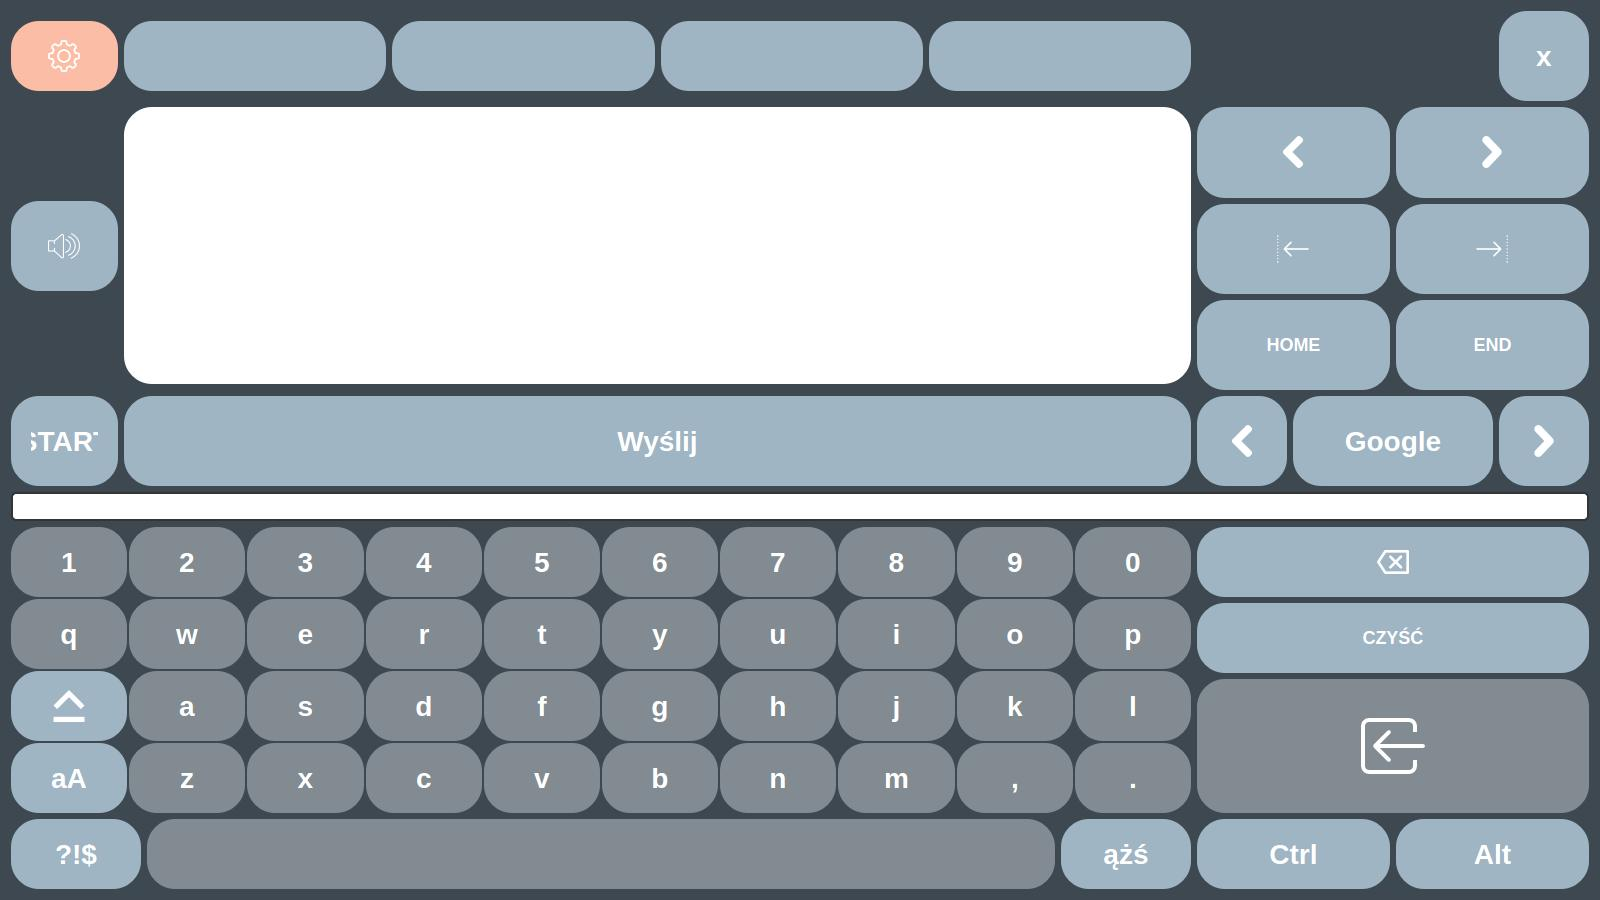
\includegraphics[width=1\textwidth]{img/main.jpg}}
		\caption{Widok interfejsu, gdy przyciski są w trybie wstrzymania.}
		\label{fig:view1}
		\end{figure}
			\begin{figure}
		\centering
		\scalebox{.7}{
		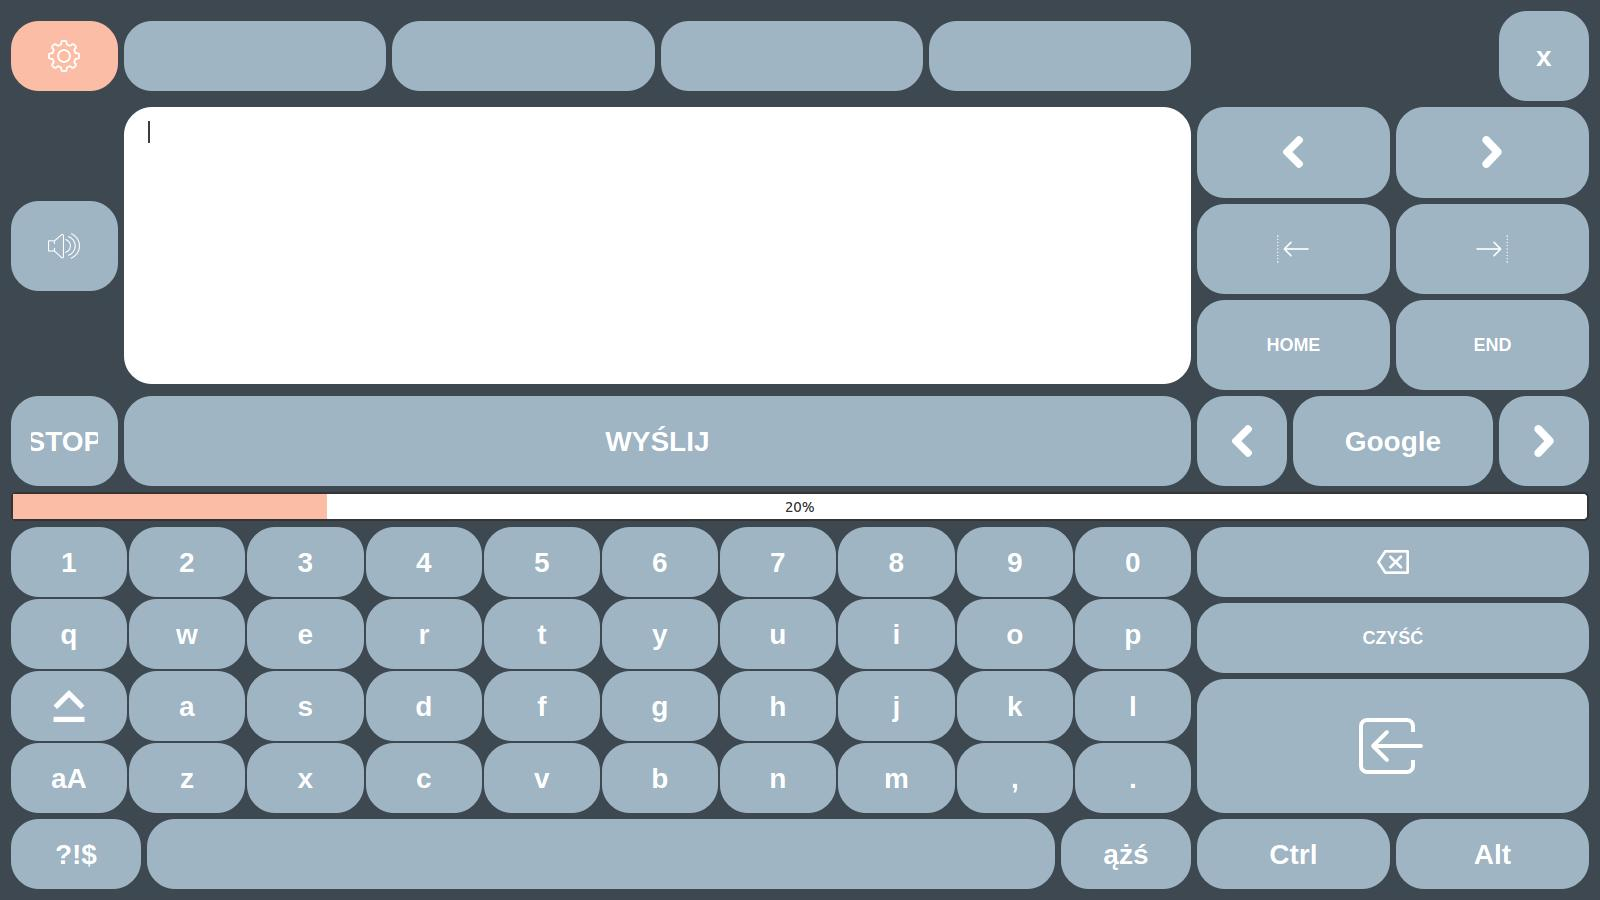
\includegraphics[width=1\textwidth]{img/stop.jpg}}
		\caption{Widok interfejsu, gdy przyciski są w trybie aktywnym.}
		\label{fig:view2}
		\end{figure}
\begin{figure}
		\centering
		\scalebox{.7}{
		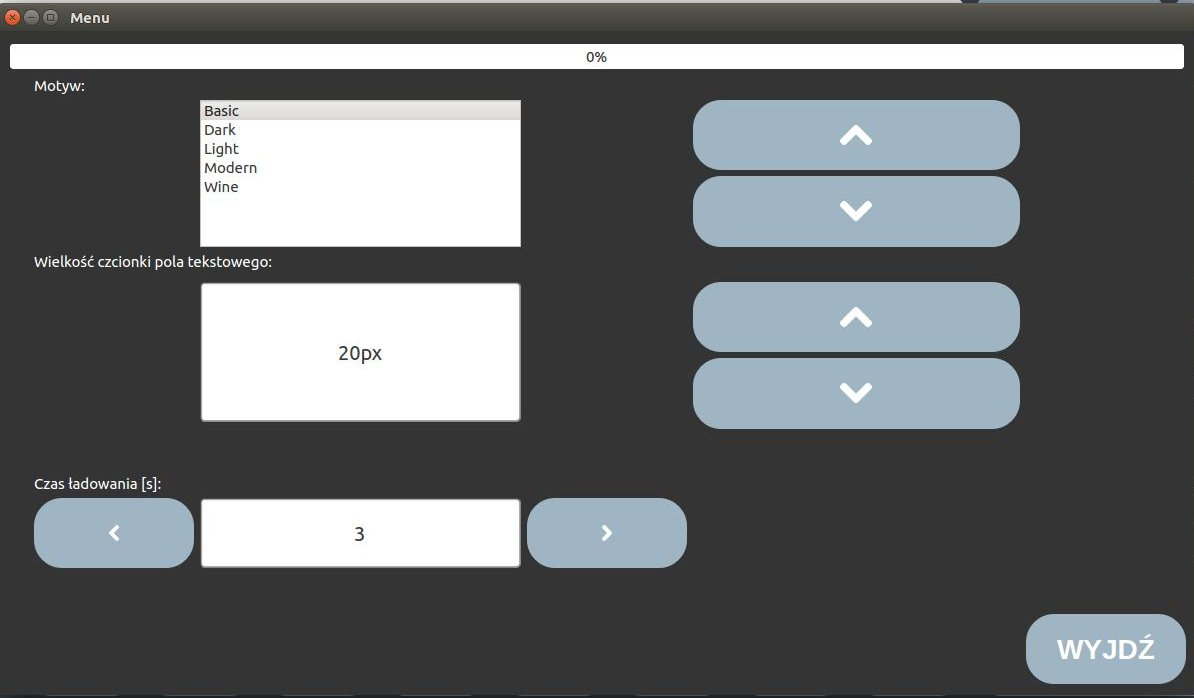
\includegraphics[width=1\textwidth]{img/menu.jpg}}
		\caption{Widok okna menu.}
		\label{fig:menu}
		\end{figure}
 Analizując widok klawiatury od górnego lewego rogu, pierwszą zmianą, którą da się zauważyć to zmina napisu ''menu'' na intuicyjną ikonę, która w sposób bardziej spójny pasuje do całościowego wyglądu. Wszystkie ikony projektu pobrane zostały ze strony ~\cite{resource} i udostępniane są na podstawie licencji CC 3.0. Autorami są Smashicons, D. Grandy, C. Fertu oraz G. Cresnar. Kolejną zmiana jest rozmieszczenie przycisków ''home'', ''end'' oraz ''czyść''. Zostały posortowane tematycznie, tak by użytkownikowi było łatwiej je odszukać. W ich miejsce przestawiony został przyciski TextToSpeech (aktualnie nieobsługiwany). W miejsce strzałek służących do poruszania się w kierunach góra-dół po tekście stworzono przyciski, których zadaniem jest przemieszczanie się po tekście o jedno słowo. Podczas testów zauważono, że przy niedługich fragmentach tekstu, do których prawdopodnie najczęściej wykorzystywana będzie klawiatura, są znacząco bardziej wykorzystywane niż strzałki góra-dół. 
Dużym ułatwieniem dla użytkownika była również zmiana dotychczas niewielkiego, kolistego paska postępu na pasek o szerokości aplikacji. Łatwiej w ten sposób obserwować zmieniajacy się stan bez odrywania wzroku od fiksowanego przycisku. Pasek dodatkowo jest w kolorze kontrastującym. 
Obok przycisku ''wyślij'', który celowo został zaprojektowany jako największy w klawiaturze (by był łatwny do trafiena i szybki w dostępie podczas konwersacji przez broadcast), pojawiły się przyciski do poruszania się po trybach wyszukiwania oraz przycisk zmieniający swój napis adekwatnie do wybranego trybu. Zmiana wygląda tak jak na rysunku ~\ref{fig:searchType}.
\begin{figure}
		\centering
		\scalebox{.7}{
		
\includegraphics[width=1\textwidth]{img/searchType.jpg}}
		\caption{Możliwe widoki trybów wyszukiwania.}
		\label{fig:searchType}
		\end{figure}


 Jak widać na rysunku ~\ref{fig:menu} użytkownikowi  do wyboru przedstawiono 5 wersji kolorystycznych interfejsu ~\ref{fig:basic},~\ref{fig:dark},~\ref{fig:light},~\ref{fig:modern}, ~\ref{fig:wine}. 
 Kolory dobrano tak, by stanowiły przyjemną do oka, spójną wizję aplikacji, a jednocześnie dawały wystaczający kontrast do  wydajnej pracy. Paletę \textit{Dark} zaprojektowano z myślą o pracy przy słabym oświetleniu, tak by jasne kolory ekranu nie raziły użytkownika w oczy. Paleta \textit{Light} przystosowana jest dla użytkowników o potrzebie mniejszego kontrastu. Zarówno kolor zielony jak i niebieski są uważane wełdug autorów publikacji ~\cite{uiColor} za barwy o charakterze relaksującym użytkownika. Palety \textit{Modern} oraz \textit{Wine} powstały w celu zwiększenia możliwości wyboru użytkownika, gdyż ostateczna ocena wyglądu intefejsu zależy od subiektywnych odczuć osoby korzystającej. Wszystkie wyżej wymienione palety powstawły w oparciu o palety stworzone na stronie ~\cite{uiColorContrast}.
 
 \begin{figure}
		\centering
		\scalebox{.7}{
		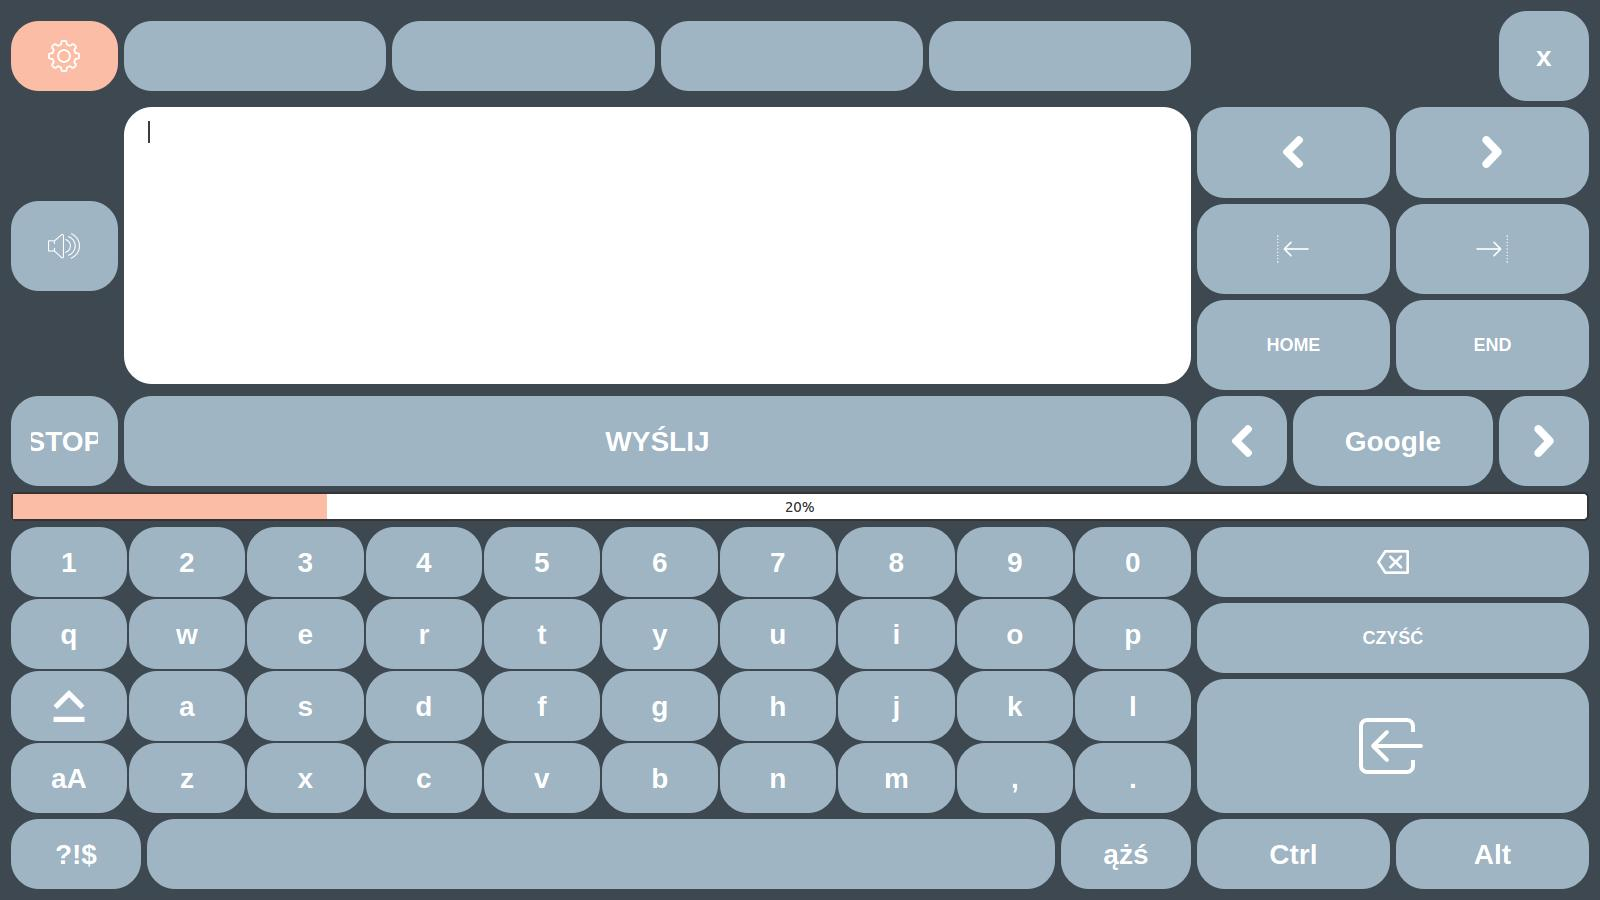
\includegraphics[width=1\textwidth]{img/stop.jpg}}
		\caption{Widok interfejsu w trybie \textit{Basic}.}
		\label{fig:basic}
		\end{figure}
		 \begin{figure}
		\centering
		\scalebox{.7}{
		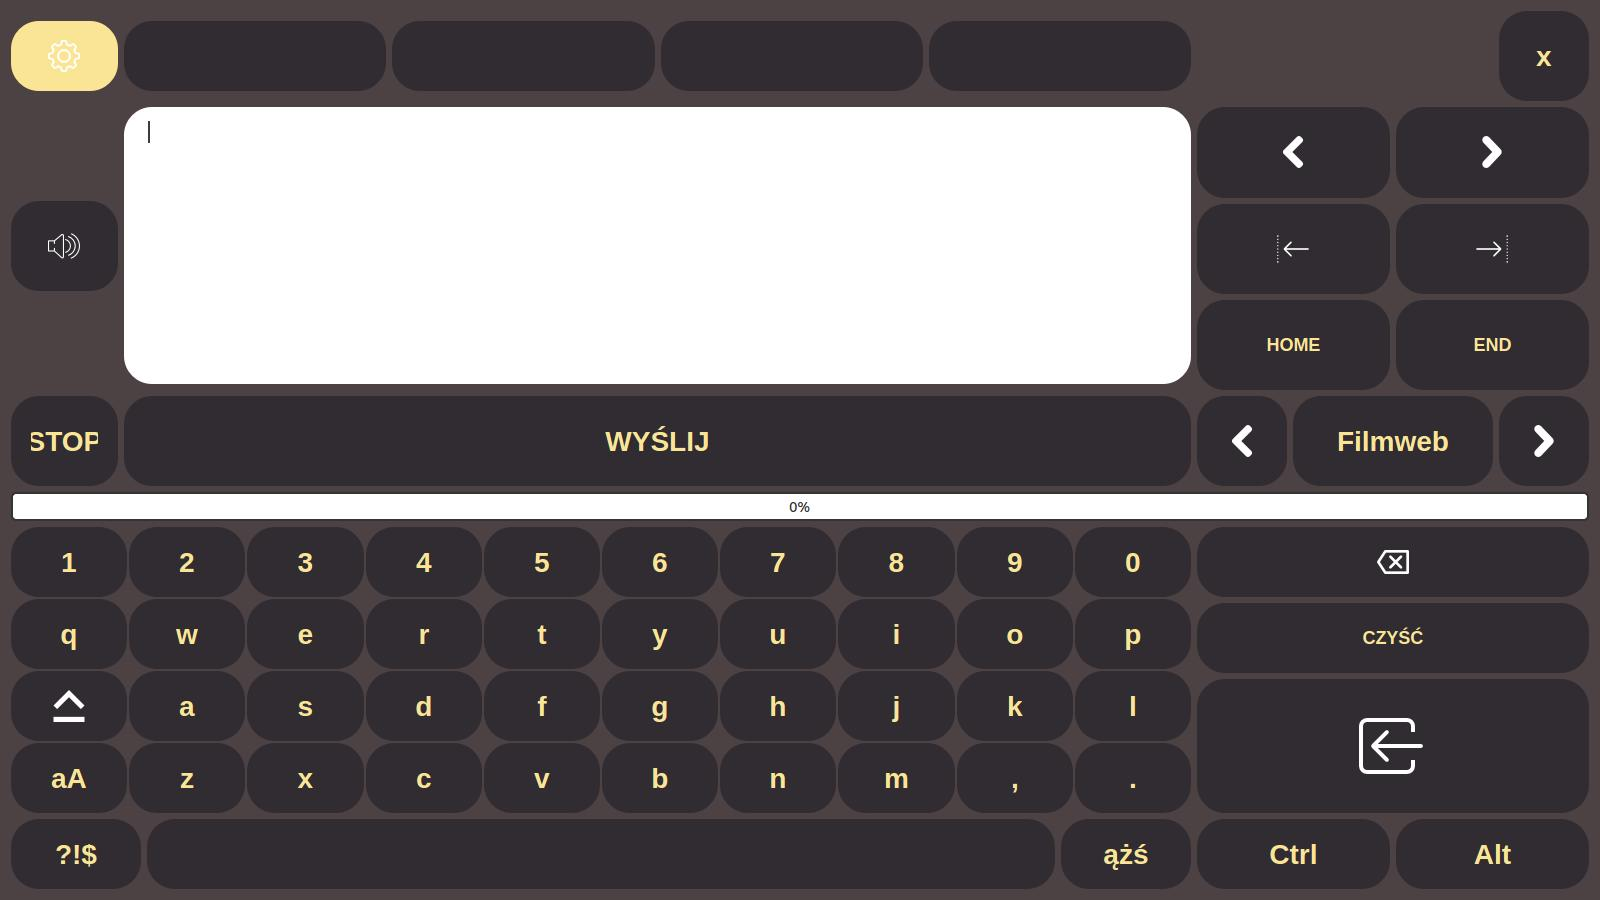
\includegraphics[width=1\textwidth]{img/dark.jpg}}
		\caption{Widok interfejsu w trybie \textit{Dark}.}
		\label{fig:dark}
		\end{figure}
		 \begin{figure}
		\centering
		\scalebox{.7}{
		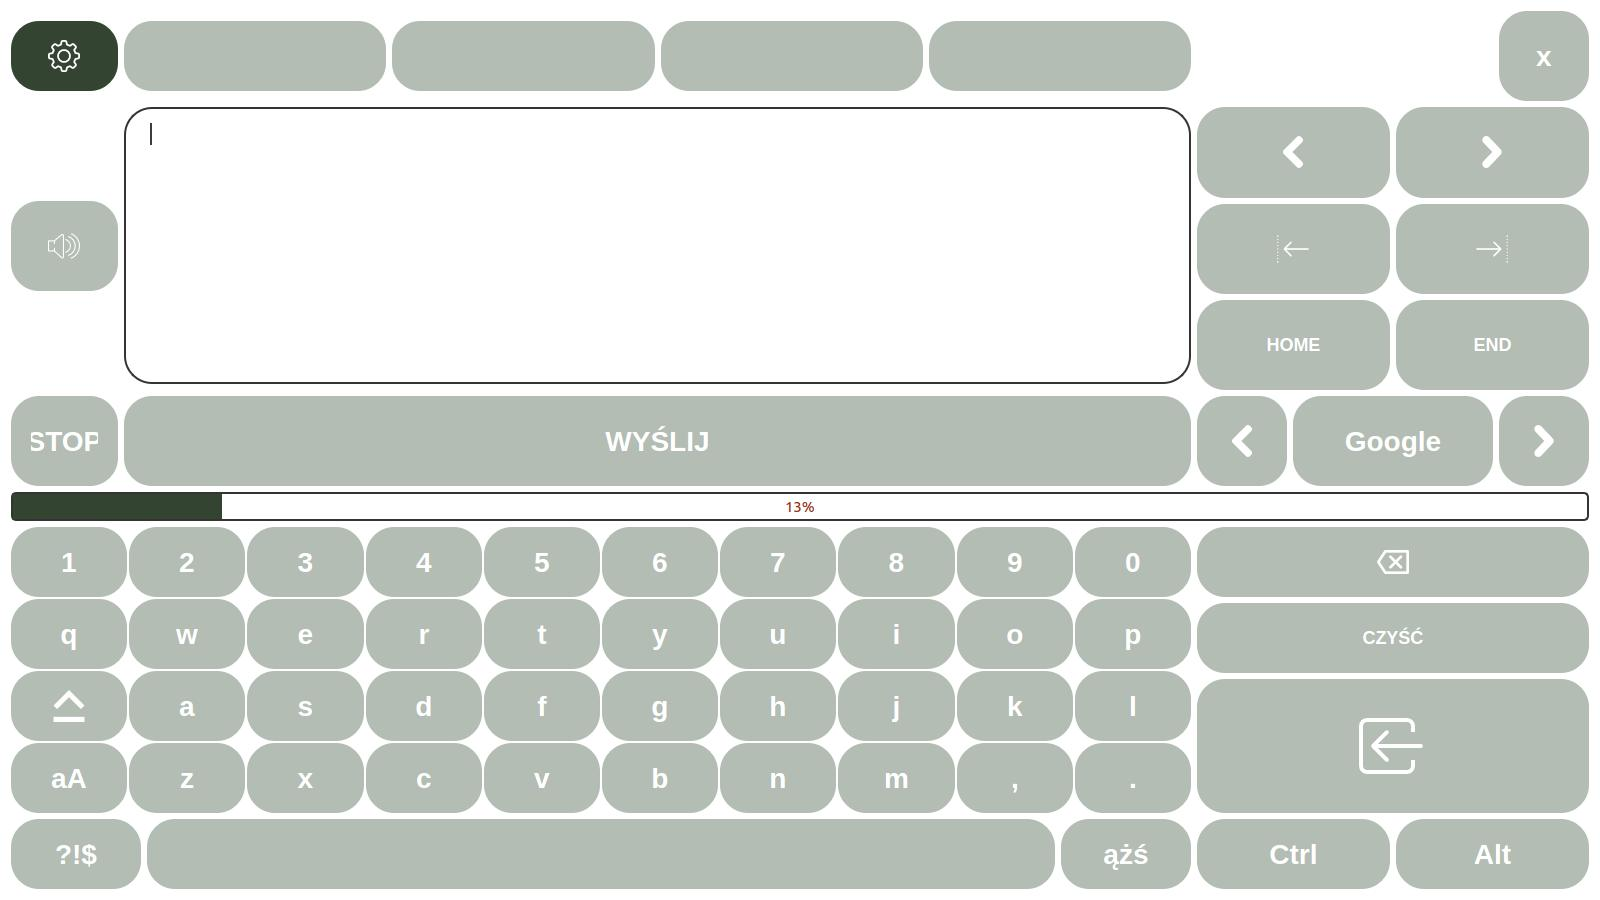
\includegraphics[width=1\textwidth]{img/light.jpg}}
		\caption{Widok interfejsu w trybie \textit{Light}.}
		\label{fig:light}
		\end{figure}
				 \begin{figure}
		\centering
		\scalebox{.7}{
		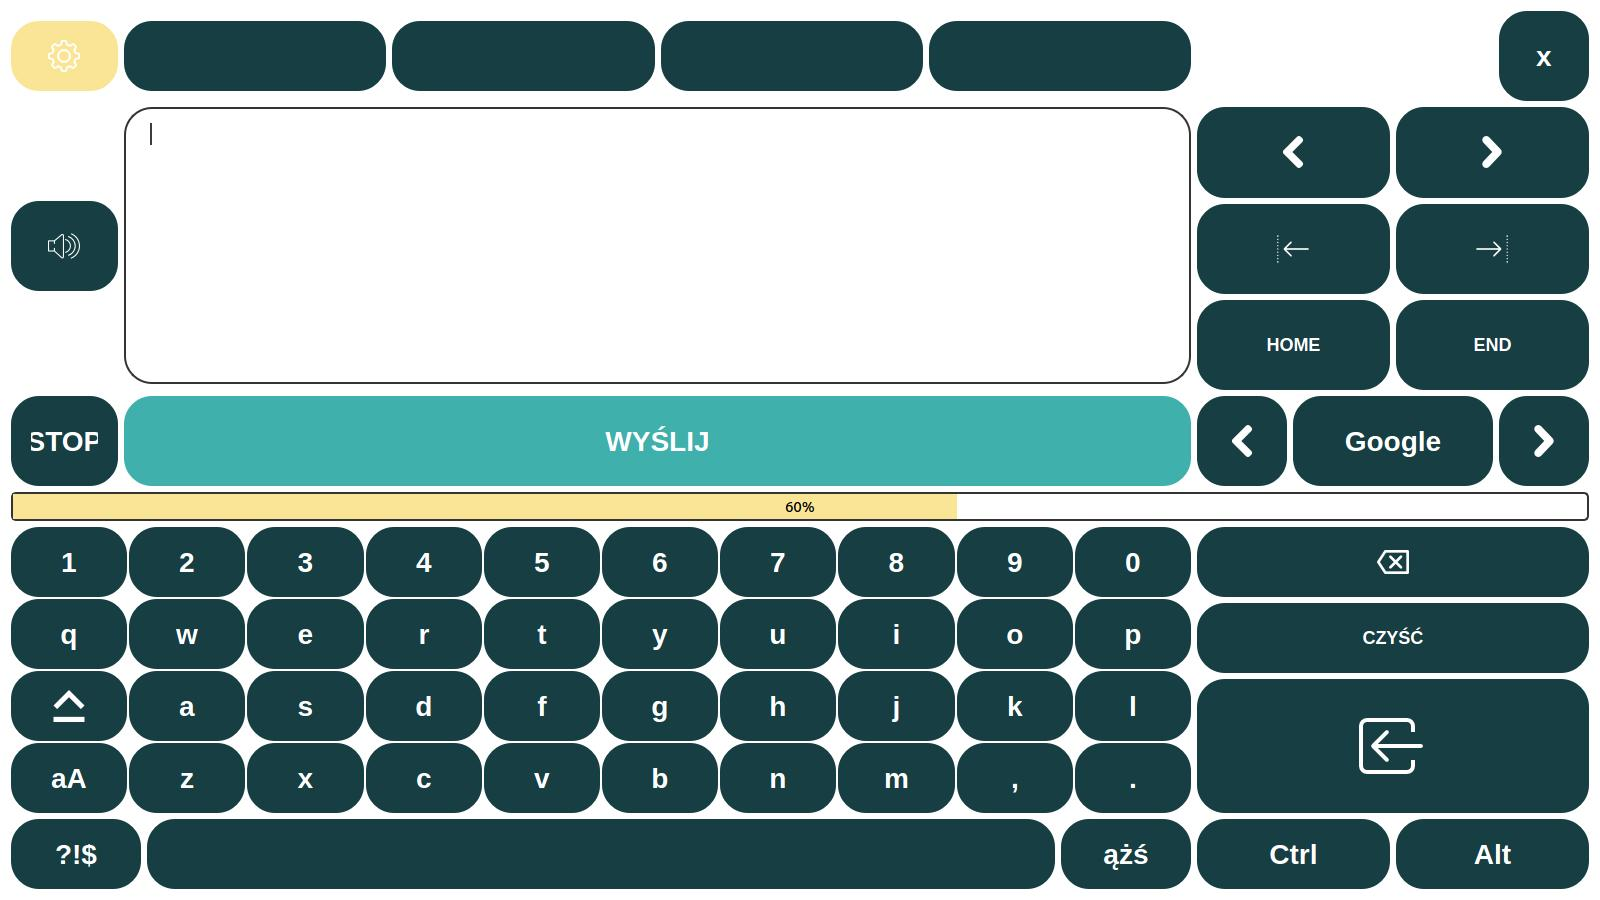
\includegraphics[width=1\textwidth]{img/modern.jpg}}
		\caption{Widok interfejsu w trybie \textit{Modern}.}
		\label{fig:modern}
		\end{figure}
		 \begin{figure}
		\centering
		\scalebox{.7}{
		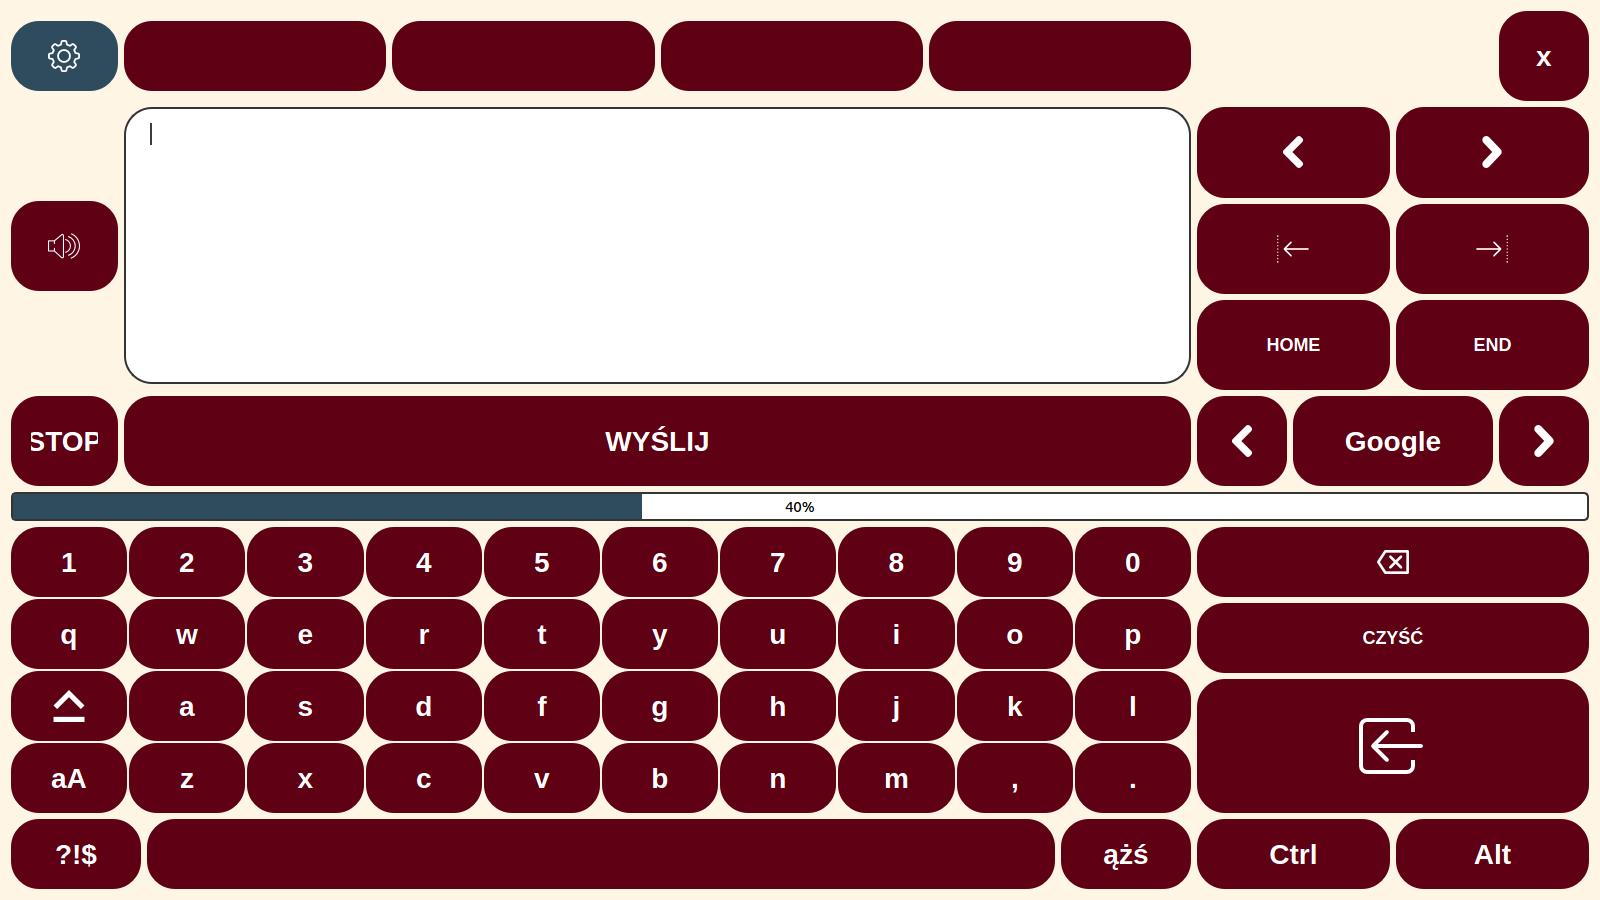
\includegraphics[width=1\textwidth]{img/wine.jpg}}
		\caption{Widok interfejsu w trybie \textit{Wine}.}
		\label{fig:wine}
		\end{figure}
\section{Podsumowanie}
W ramach relizacji projektu udało się zaimplementować wszystkie zaplanowane w rodziale ~\ref{sec:chap3} funkcjonalności. Niektóre zachowania zostały zmienione (np. wybór trybu wysyłania/wyszukiwania) względem zaplanowanych na diagramie przypadków użycia ~\ref{sec:uml}. Wynikło to z analizy sposobu korzystania z przycisków klawiatury i uznano nowy rozkład za bardziej ergonomiczny. Działanie oprogramowania omówiono w powyższym rozdziale ze szczegółowym opisem zastosowanych algorytmów bazowych,dzięki którym możliwe jest popranwe działanie aplikacji. Wymieniono i wytłumaczono rolę najważniejszych zmiennych. Omówiono nowy wygląd intefrejsu użytkownika oraz powody, dla których wprowadzono różnice w porównaniu z prototypem.  

 \end{document}
 